\documentclass{beamer}
\usepackage{graphicx}
\usepackage{paralist}

\author{Joshua Paul Barnard}
\title{Who is your Instructor?}
\titlegraphic{\vspace{-10mm}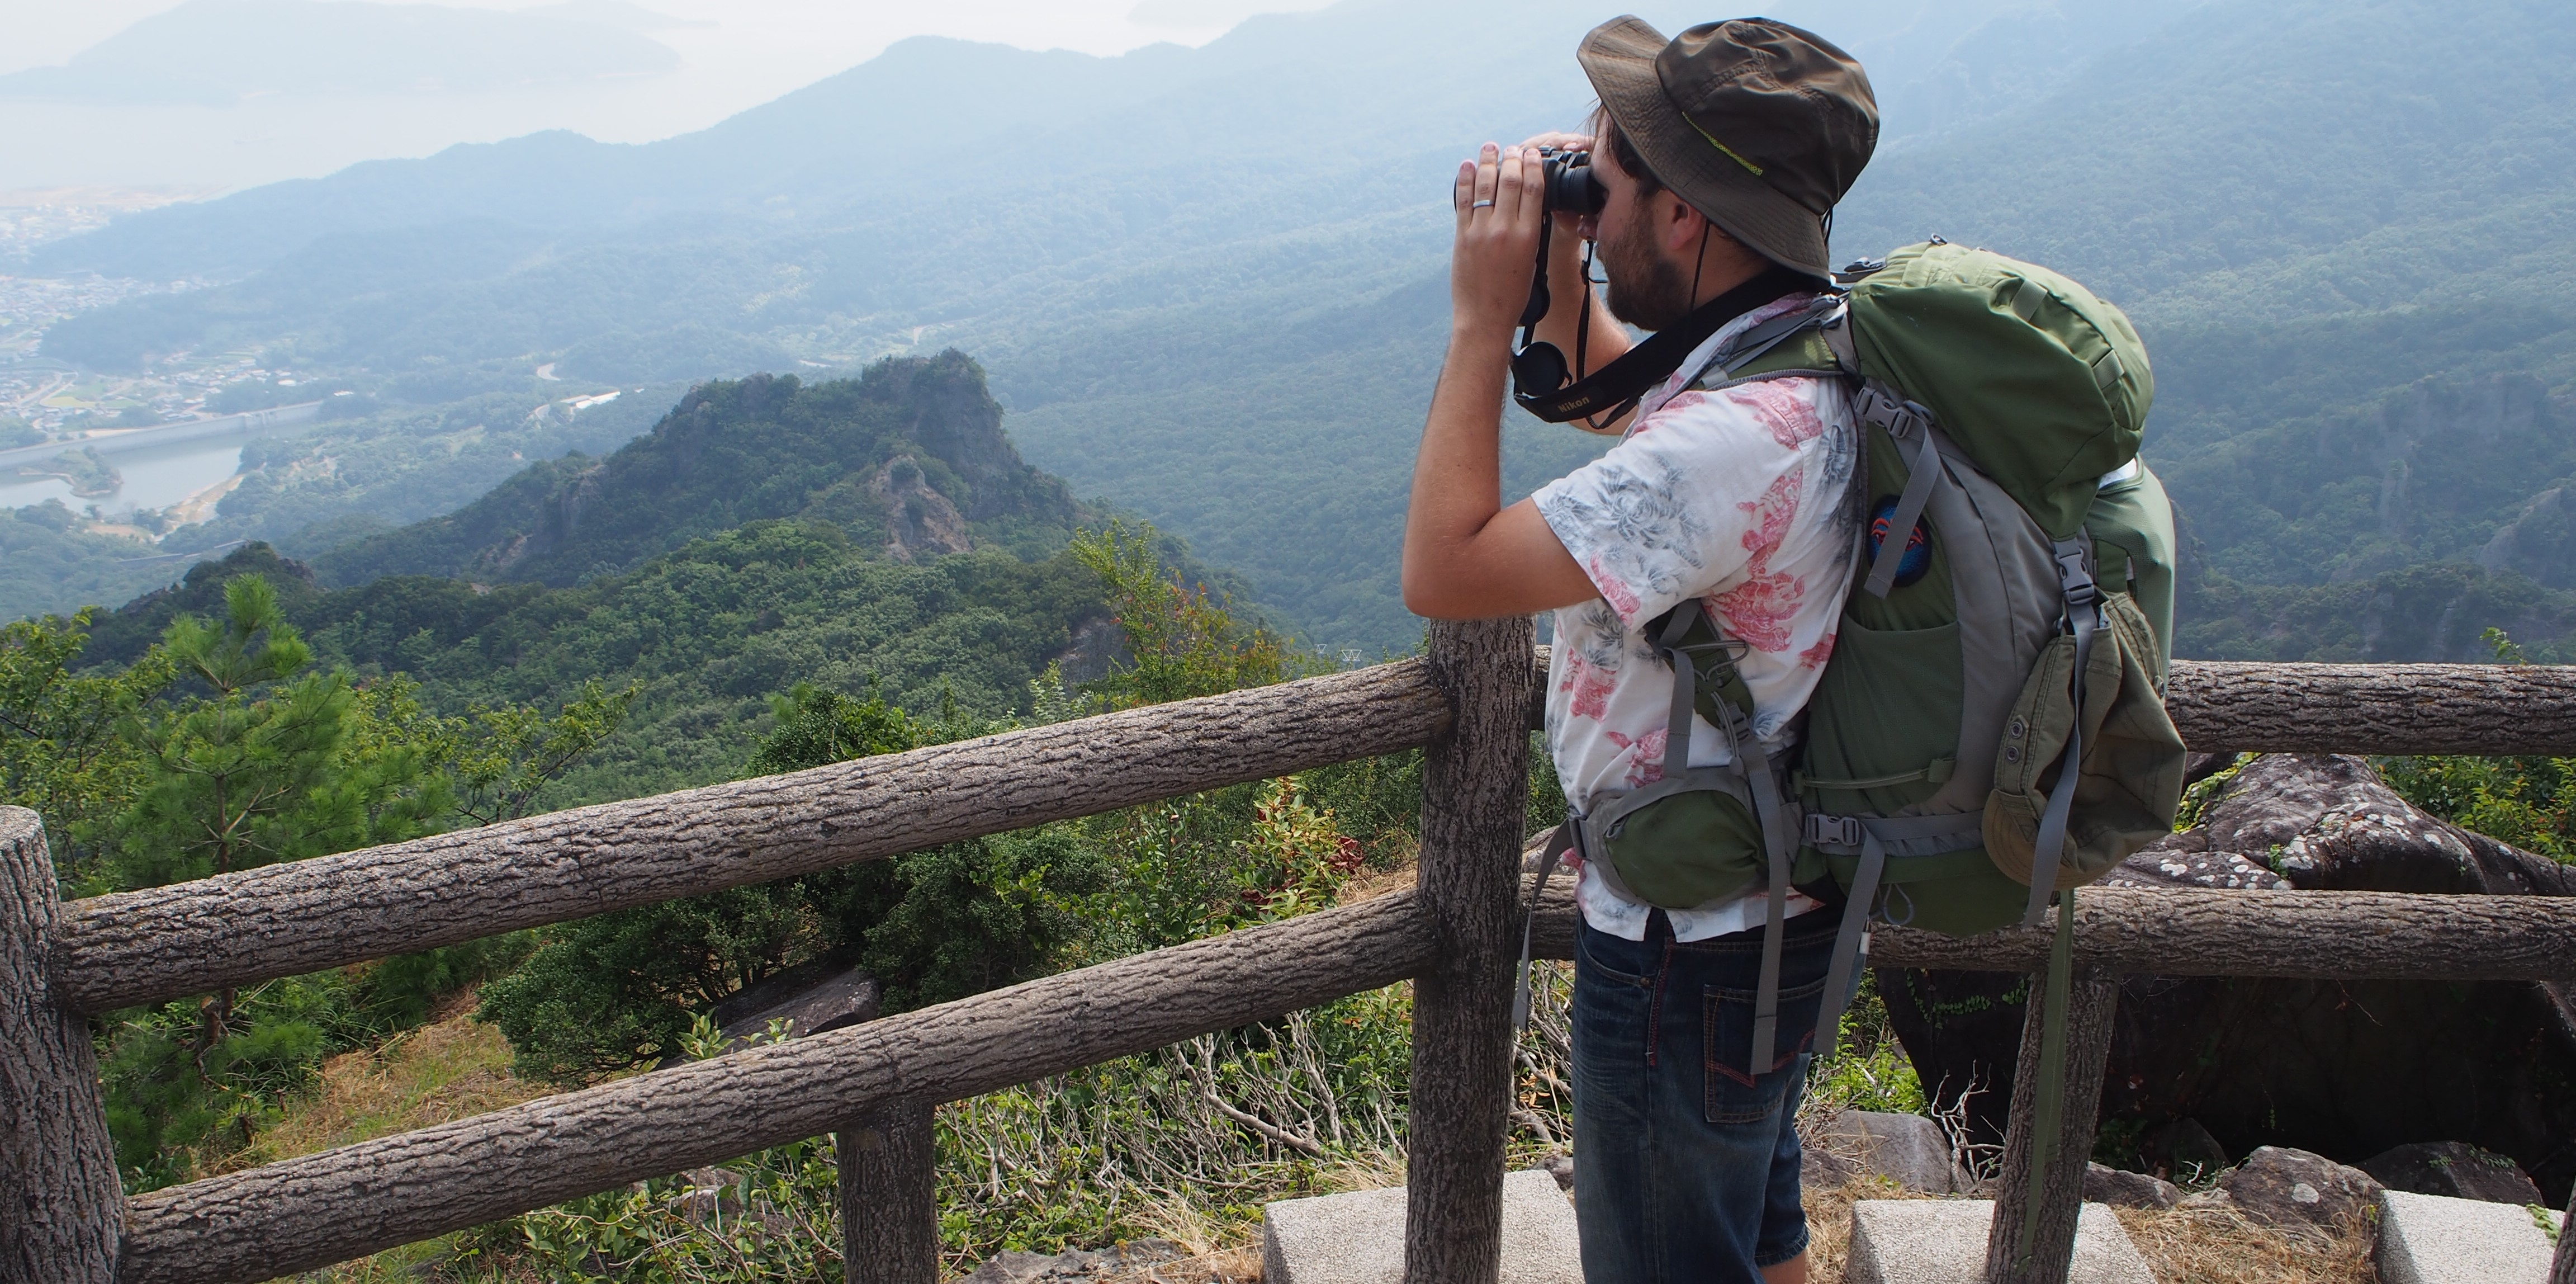
\includegraphics[width = .8\textwidth]{images/P8154828.jpg}} 
\date{\vspace{-5em}} 


\mode <presentation>
\usetheme{Warsaw}
\usecolortheme{default}

\setbeamerfont{footline}{size=\fontsize{5}{8}\selectfont}

\definecolor{darkred}{rgb}{20,0,0}
\definecolor{darkgreen}{RGB}{40,110,20}
\definecolor{darkpurple}{RGB}{30,0,30}
\definecolor{chardonnay}{RGB}{255, 255, 204}

\setbeamercolor*{palette primary}{fg=white, bg=darkgreen}


\begin{document}
	{
		\setbeamertemplate{footline}{} 
		\setbeamertemplate{headline}{} 
		\begin{frame}
			\vspace{-35pt}
			\maketitle
		\end{frame}
	}


	\section{ About Me }

		\subsection{About Me}
		
				\begin{frame}
			\frametitle{About Me}
			\begin{itemize}
				\item 36 years old, male
				\item Northern California Coast Native
			\end{itemize}
			\begin{center}
				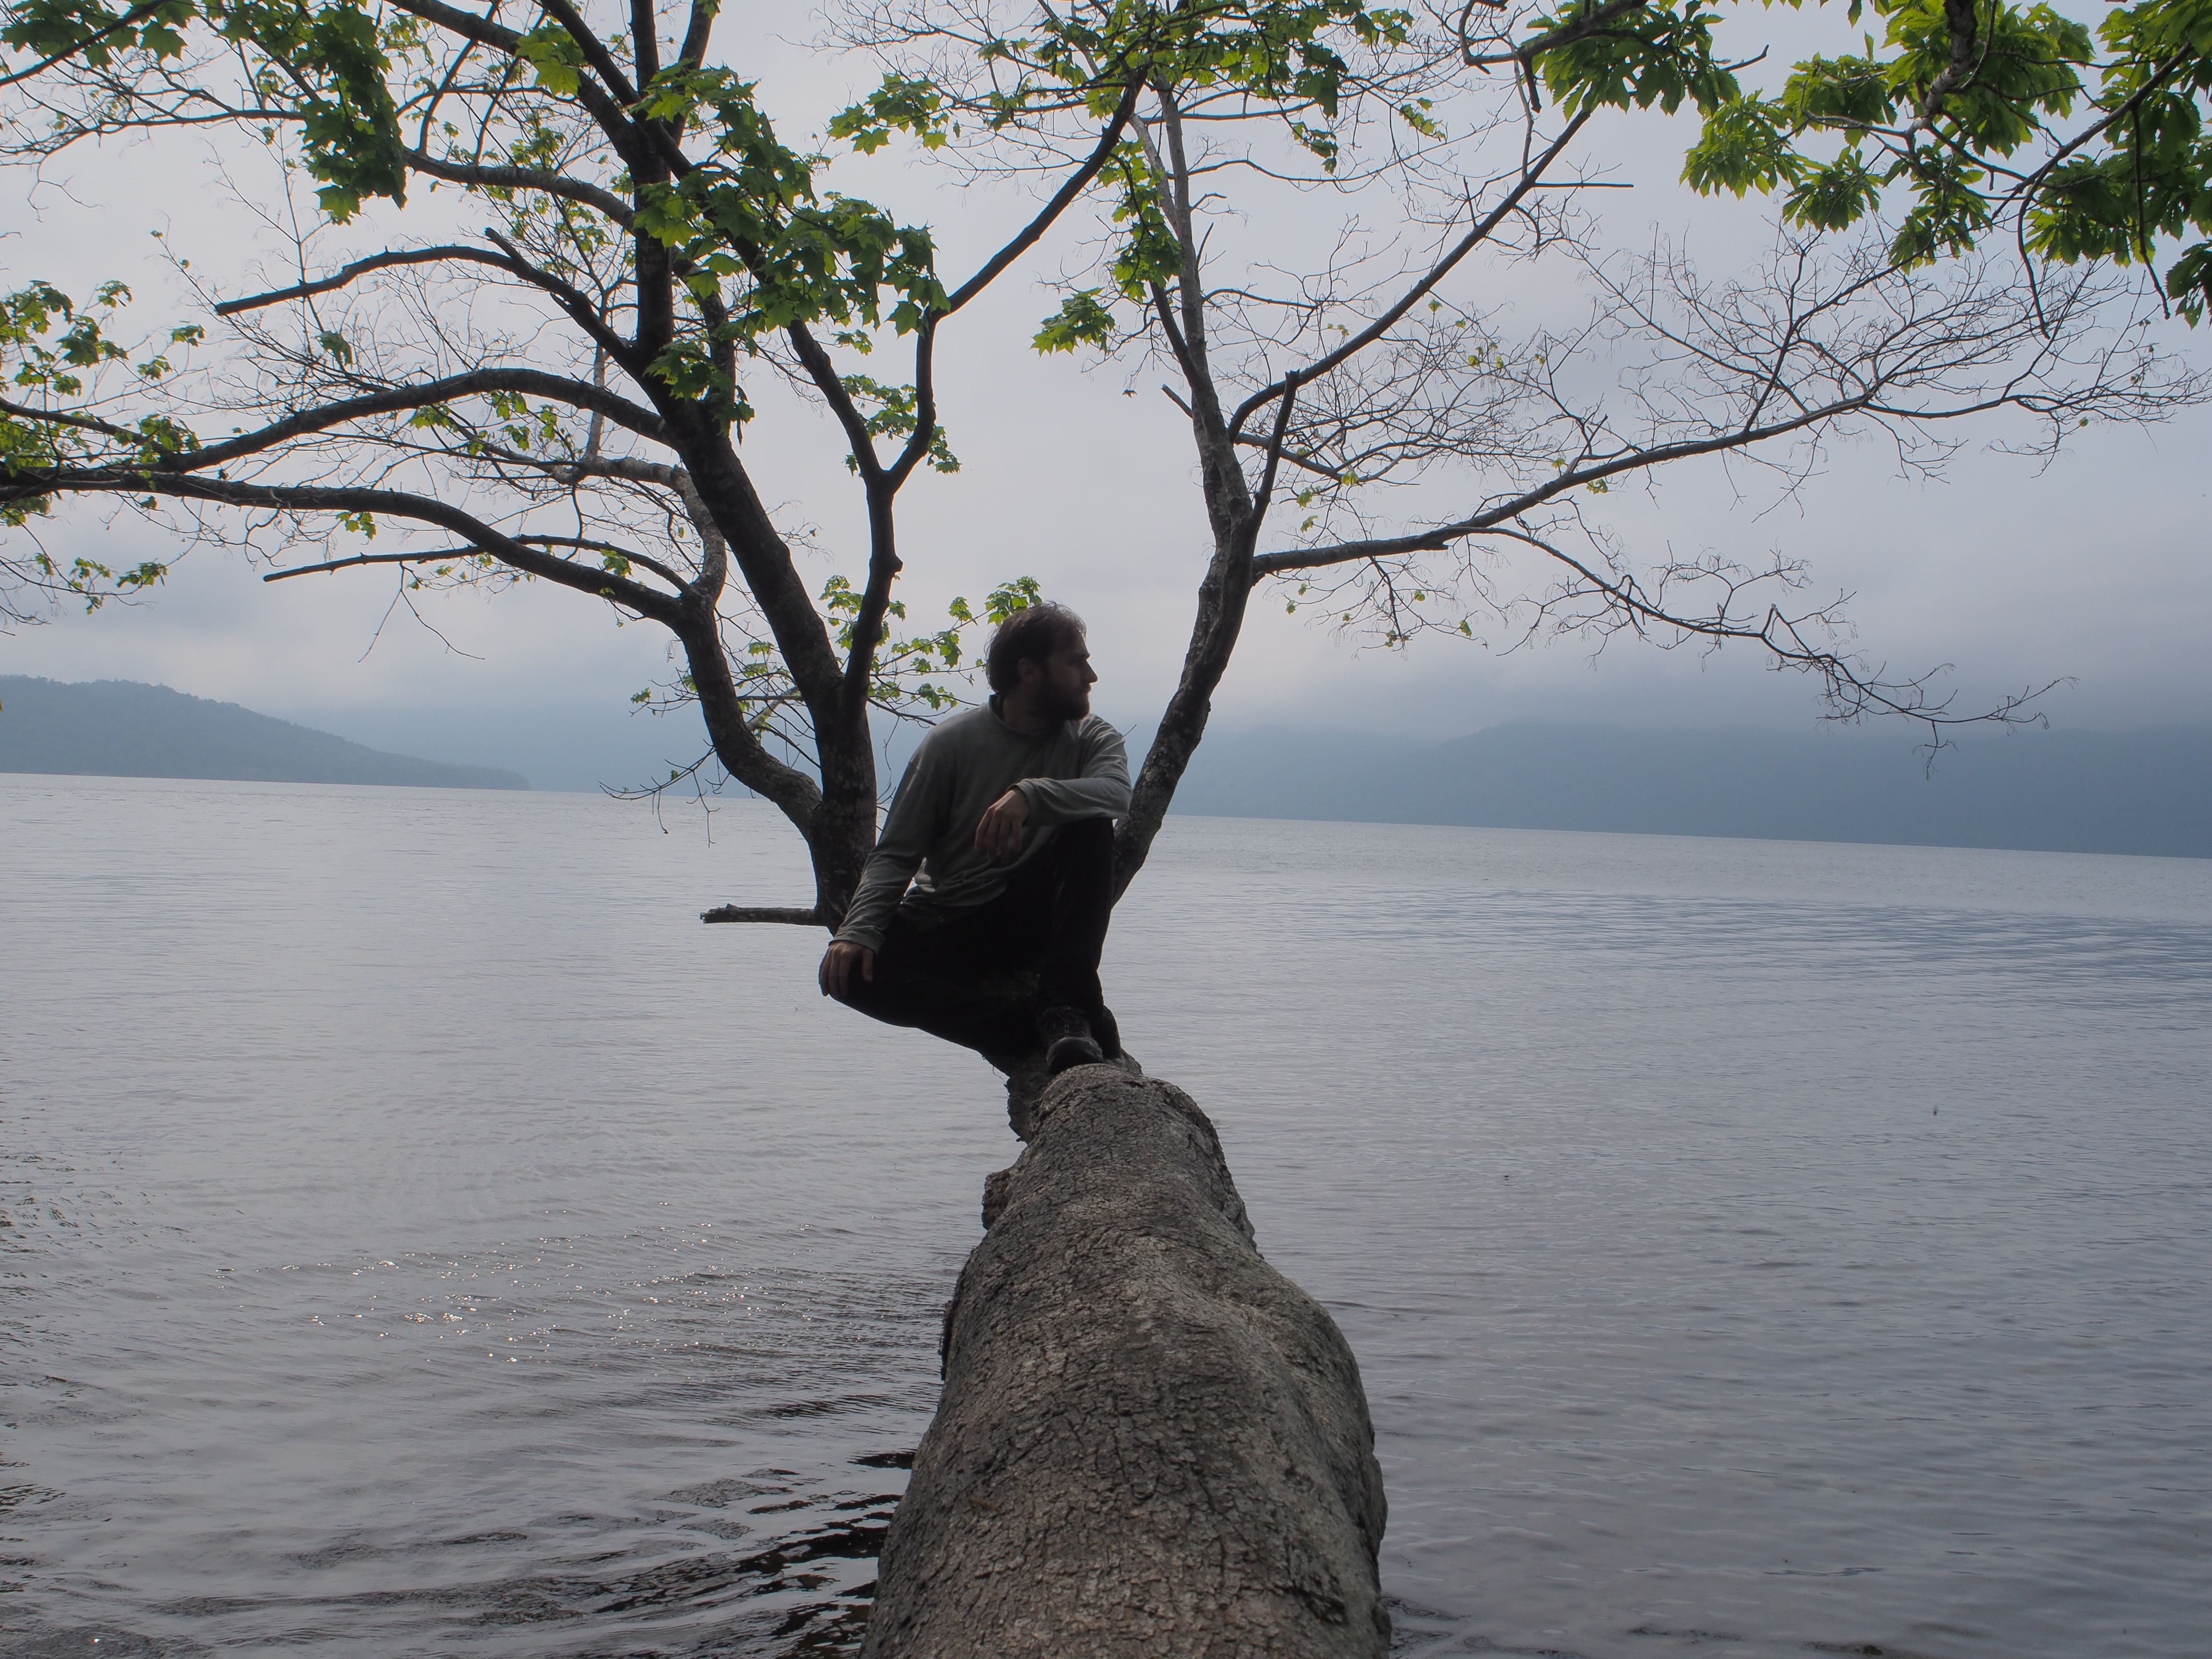
\includegraphics[width = 1.0\textwidth]{images/P6190078.JPG}
			\end{center}
		\end{frame}
	
	\subsection{Where I am From}
	
		\begin{frame}
			\frametitle{Where am I from?}
				\begin{itemize}
					\item Born and Raised in Santa Rosa, California.  
					\item From Telecom Valley and the Sonoma/Napa Wine Region.
					\item Family on my Mothers side is from Fort Bragg, California
					\end{itemize}
				\begin{center}
					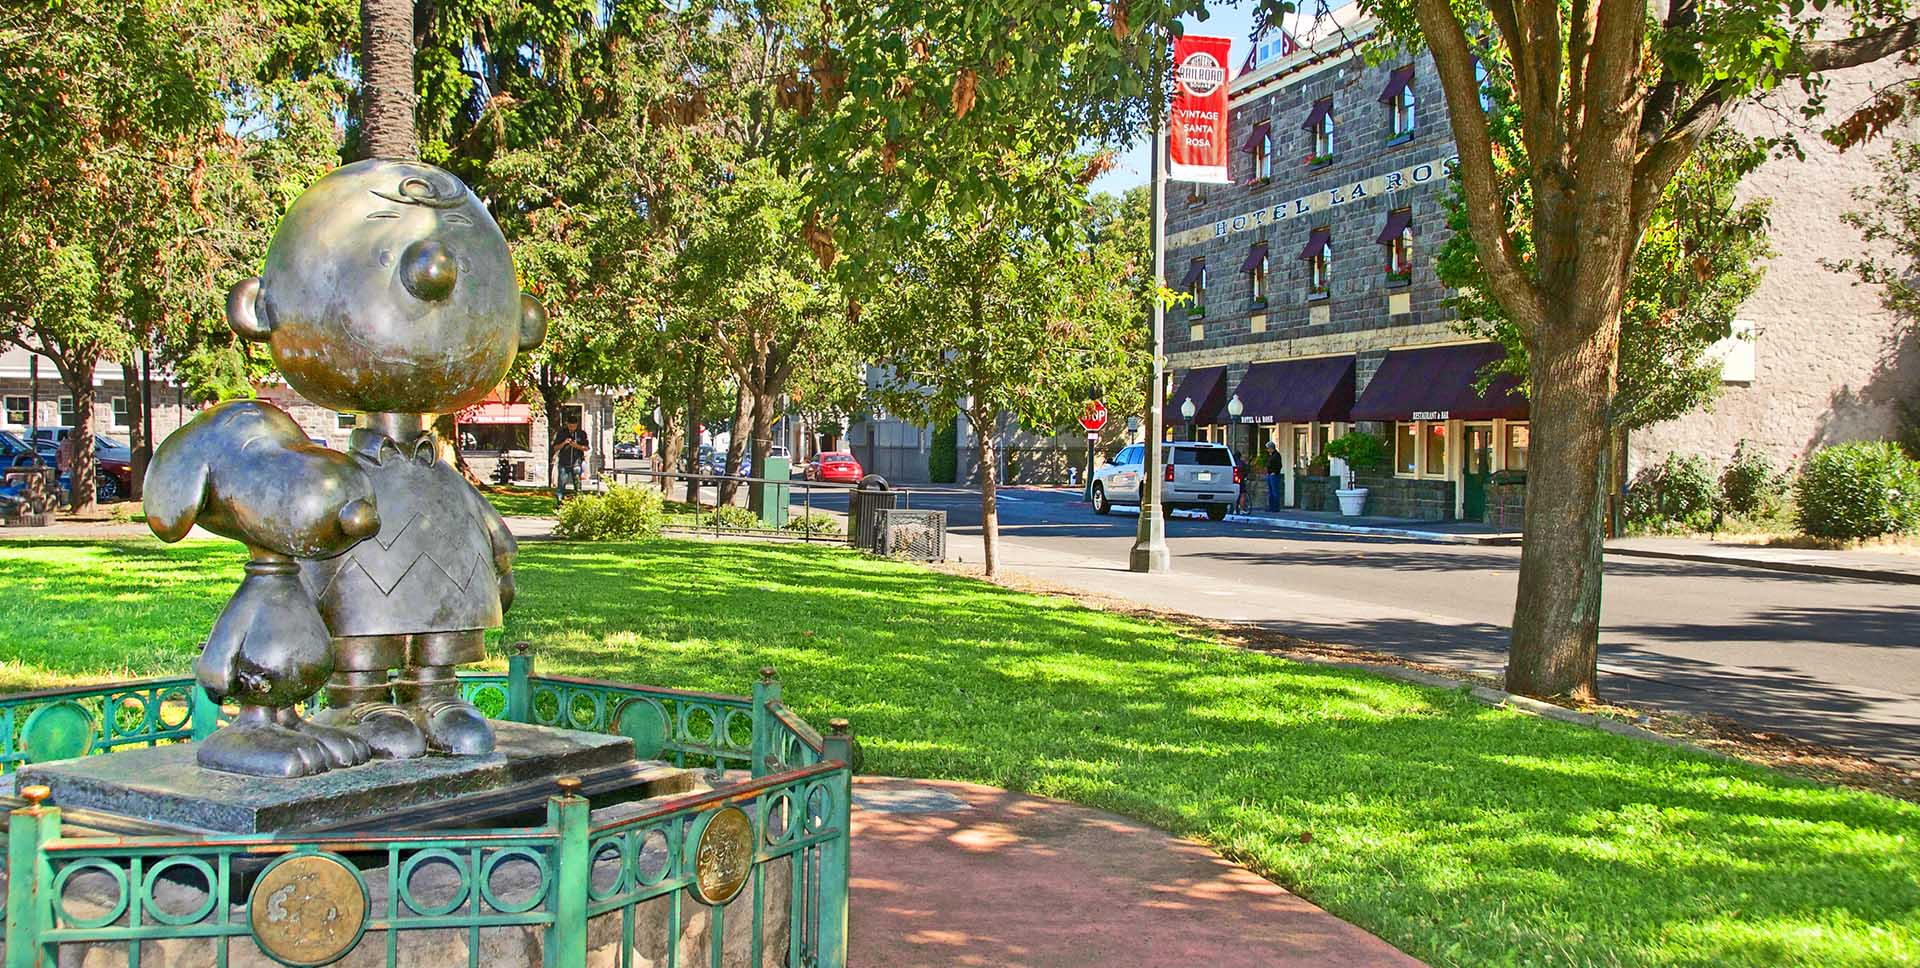
\includegraphics[width = 1.0\textwidth]{images/santa_rosa_1920x968.jpg}
				\end{center}
		\end{frame}
	
			\begin{frame}
		\frametitle{Where Have I Lived?}
		\begin{itemize}
			\item Sonoma, Mendocino, \& Humboldt Counties in California.  
			\item Nagoya, in Japan.  
		\end{itemize}
		\begin{center}
			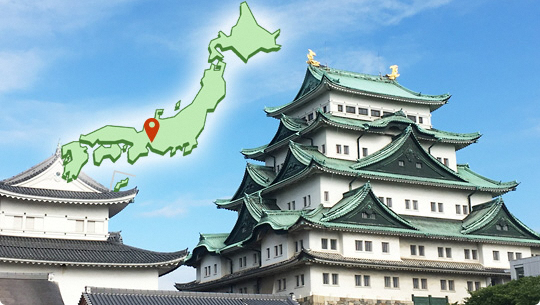
\includegraphics[width = 1.0\textwidth]{images/nagoya.png}
		\end{center}
	\end{frame}
	
	
		\subsection{My Family}
		
			\begin{frame}
	\frametitle{My Parents}
	\begin{itemize}
		\item My Mother was an Elementary School Teacher, Psychiatric Technician, and Caregiver.
		\item She is currently 74 years old and retired.
		\item My Father had a PhD in Psychology, and was a Supervising Psychiatric Technician.  
	\end{itemize}
	\begin{center}
		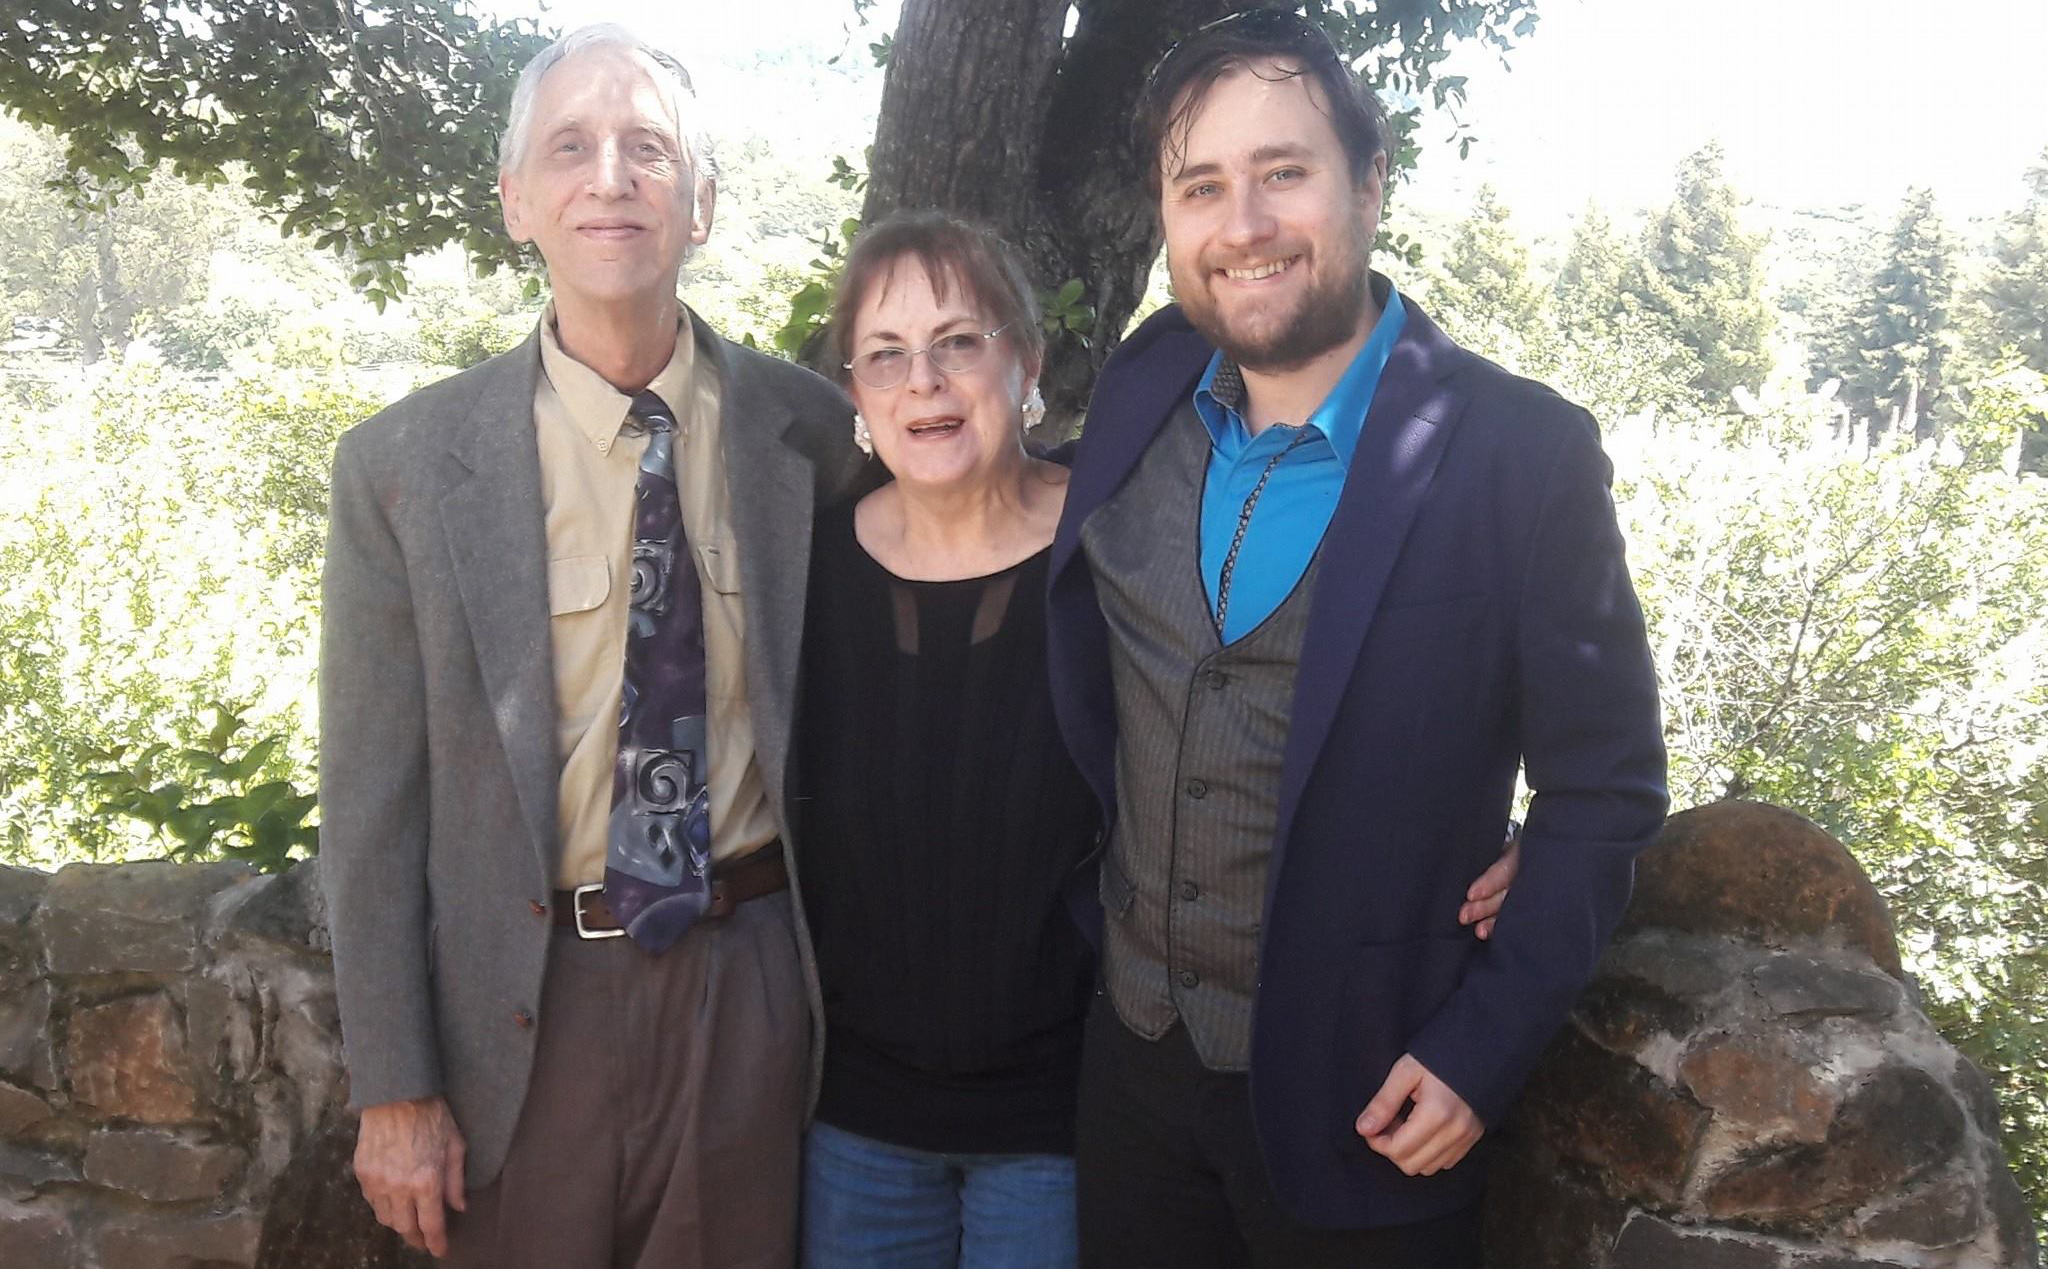
\includegraphics[width = 1.0\textwidth]{images/parents.png}
	\end{center}
\end{frame}
		
			\begin{frame}
				\frametitle{My Wife}
				\begin{itemize}
					\item My wife and I met while I was traveling around Japan during a summer break from University.
					\item She is from the city of Chengdu
					\item We got married in Nagoya, Japan on July 2nd, 2017.
				\end{itemize}
				\begin{center}
					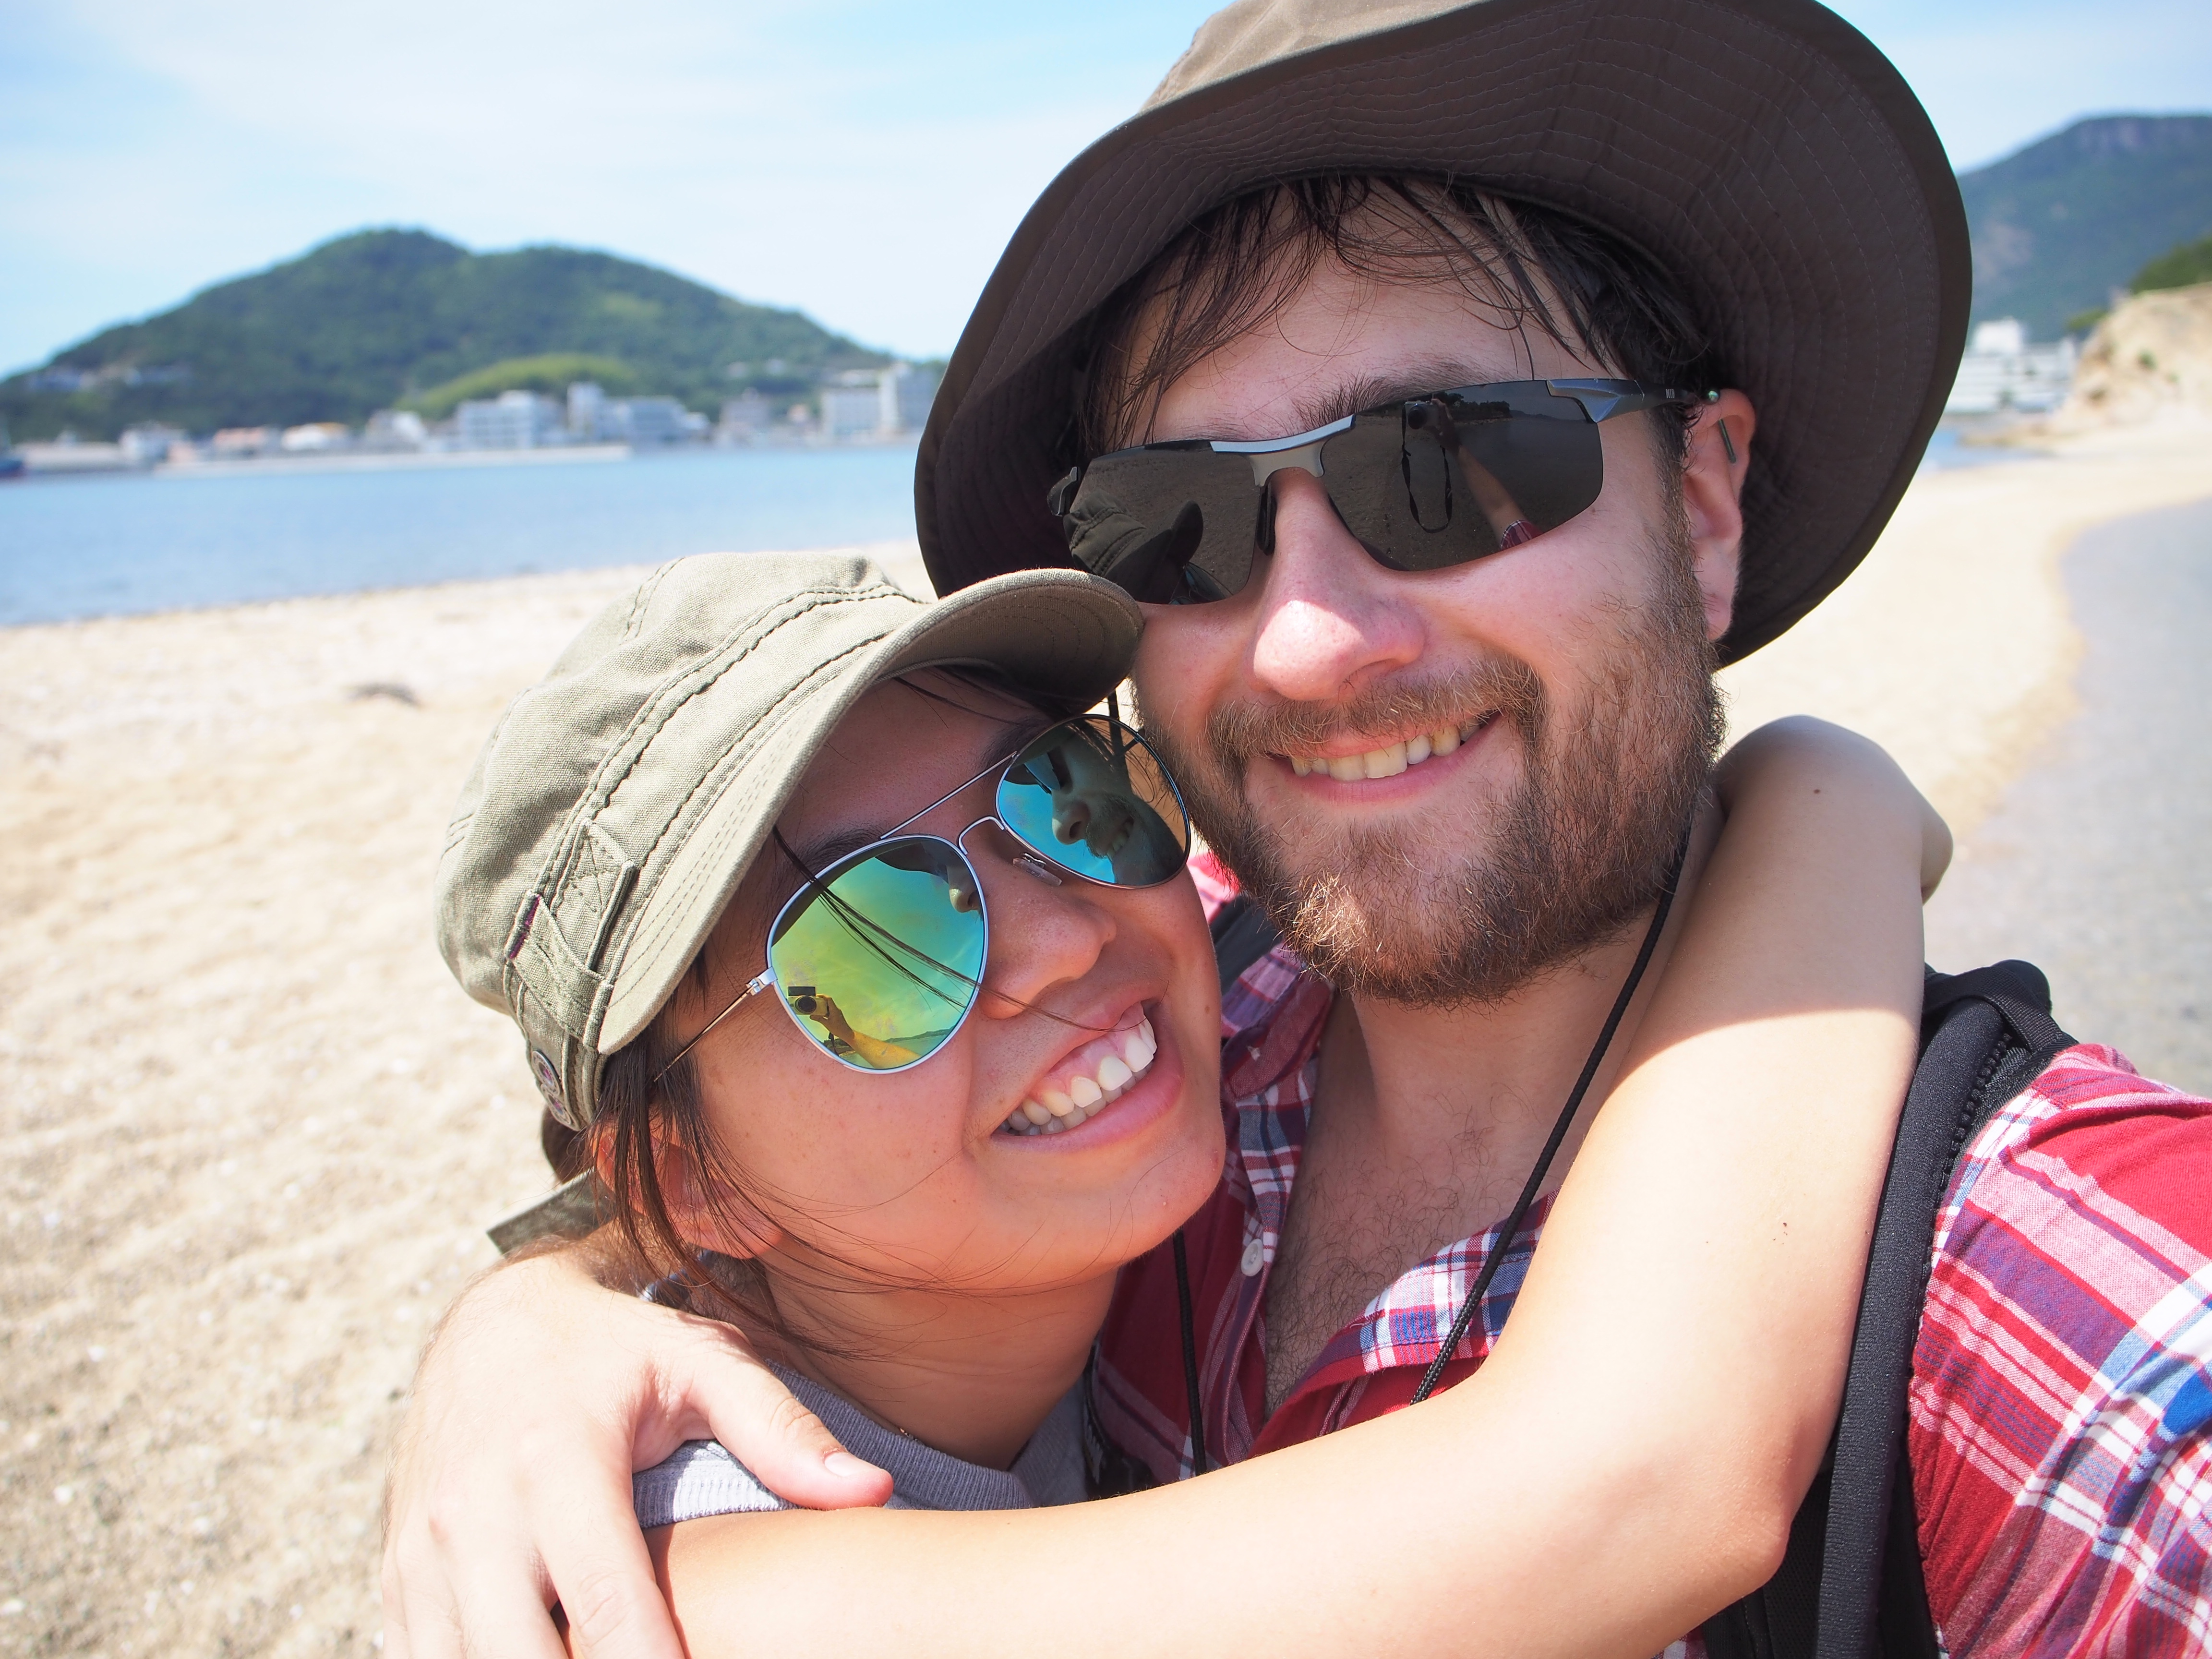
\includegraphics[width = 0.7\textwidth]{images/P8114378.JPG}
				\end{center}
			\end{frame}
		
			\begin{frame}
							\frametitle{Our Dogs}
								\begin{itemize}
					\item We got Michio (the white dog) the day we got back to California from Japan.
					\item Sequoia (the black dog) is from a foster home up in Yreka, California.
				\end{itemize}
				\begin{center}
					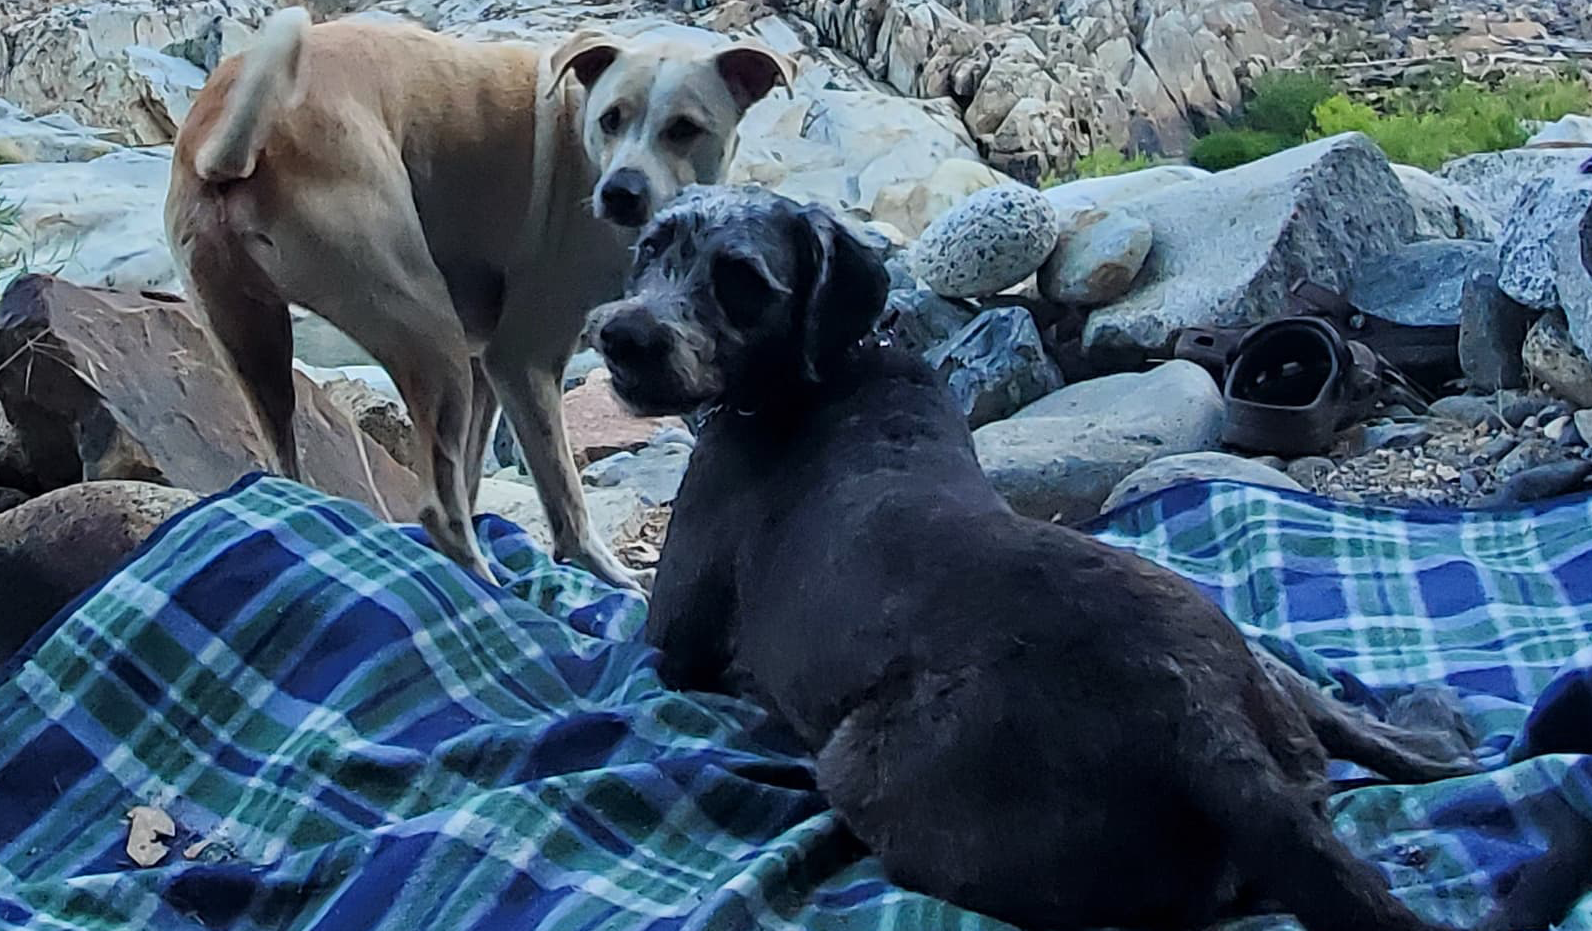
\includegraphics[width = 0.9\textwidth]{images/michio and sequoia.png}
				\end{center}
			\end{frame}
		
			\begin{frame}
	\frametitle{Our Orchard}
	\begin{itemize}
		\item We live on my grandparents property, 5 miles outside of Fort Bragg, California.
		\item Planted a small garden and orchard, consisting of 15 fruit/nut trees and various berries, herbs, spices and flowers.   
	\end{itemize}
	\begin{center}
		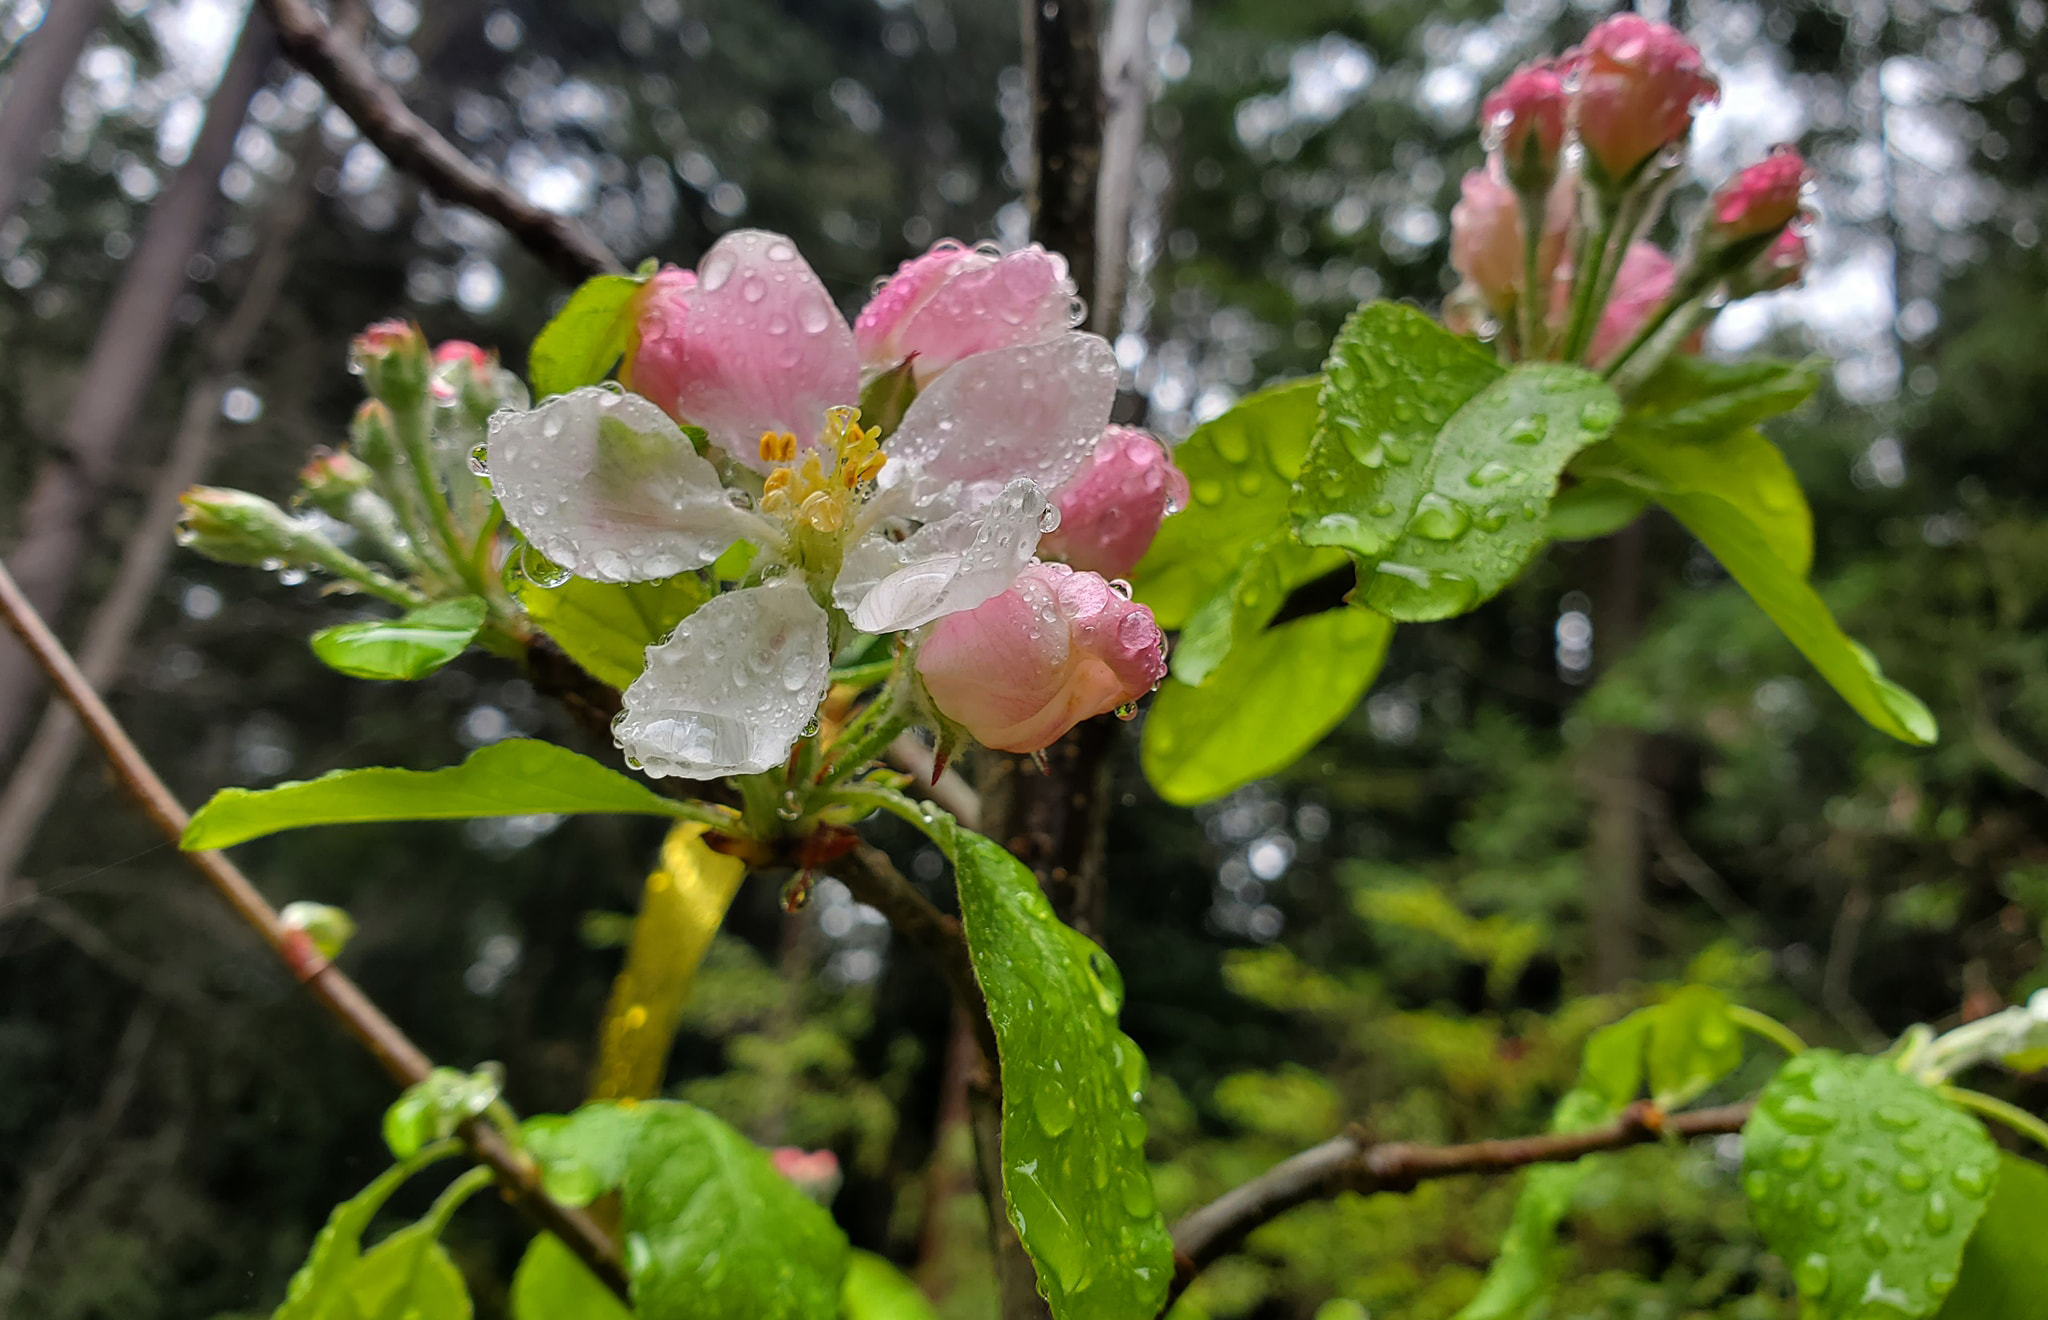
\includegraphics[width = 1.0\textwidth]{images/flower.png}
	\end{center}
\end{frame}
			
			
		\subsection{What I am doing}
			\begin{frame}
				\frametitle{What I'm Doing Now}
				\begin{itemize}
					\item Graduate Student with Johns Hopkins University.
					\item Computer Science Instructor with Mendocino College
					\item Making my own business, to provide accommodations, \& sell plants and food.     
				\end{itemize}
				\begin{center}
					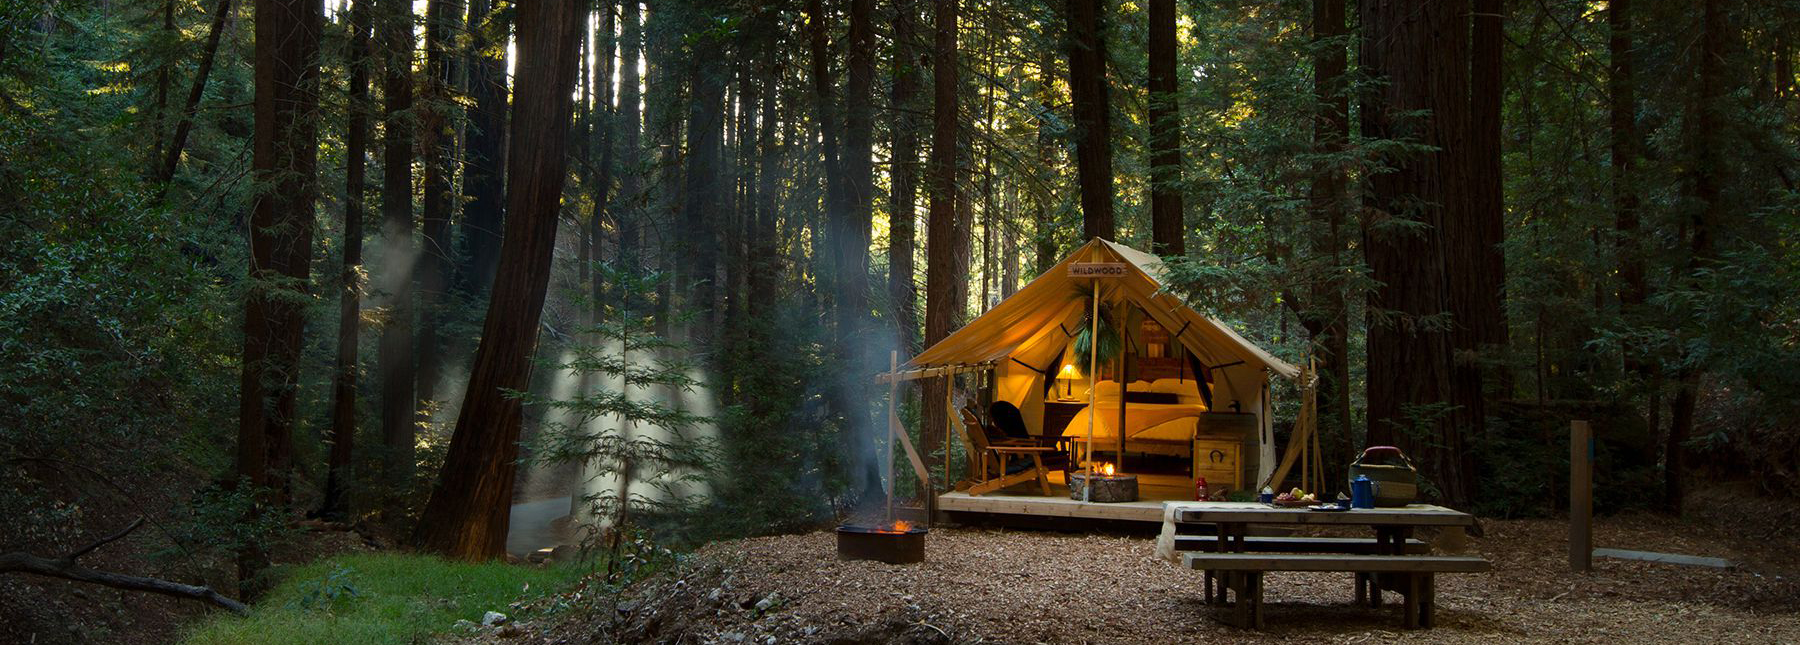
\includegraphics[width = 1.0\textwidth]{images/glamping.png}
				\end{center}
			\end{frame}



	\section{Education \& Career}
	
		\subsection{High School \& Tutoring}
			\begin{frame}
				\frametitle{My High School Experience}
				\begin{itemize}
\item My parents setup our home as a school, as my dad had a PhD in Psychology and my Mother had been a elementary school teacher.  
\item I attended the Santa Rosa Junior College under the High School Enrichment Program
\item I am in the freshman yearbook for Maria Carrillo High School.  
\item Was active in Boy Scouts, a church youth group, and even attended high school prom. 
\item At the age of 18 I earned my first Associate Degree.  
				\end{itemize}
				\begin{center}
					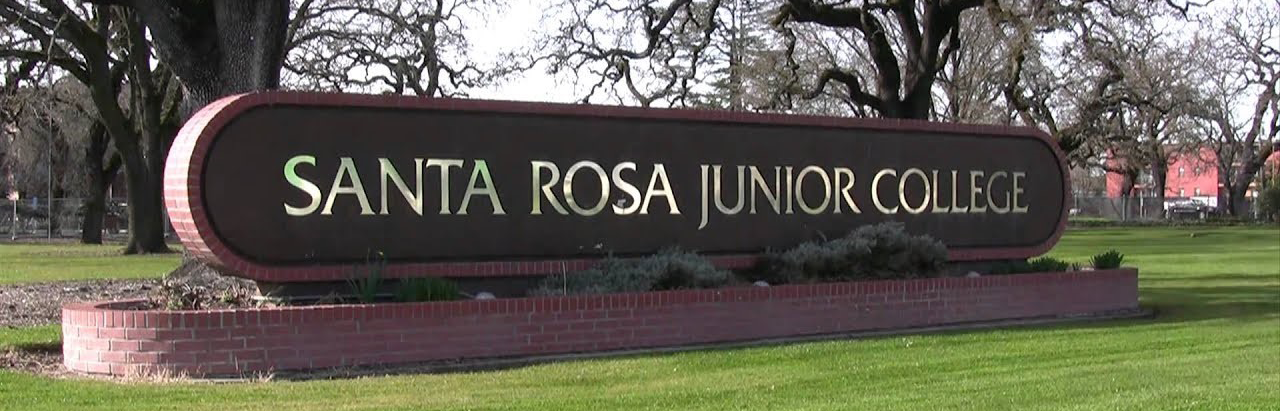
\includegraphics[width = 1.0\textwidth]{images/SRJC_sign.png}
				\end{center}
			\end{frame}
		

\begin{frame}
	\frametitle{How I Started Tutoring}
	\begin{itemize}
		\item Started tutoring fellow students in my introductory computer classes at the age of 15.  
		\item Began work at the Santa Rosa Junior College's Tutorial Center at the age of 16.
		\item Math Lab Drop-in and scheduled one-on-one tutoring sessions.  
		\item Primary Subjects:  Mathematics (Algebra and Statistics), and Computer Science.
		\item Additional Subjects:  Psychology, Web Development, Game Programming, Graphic Arts.
	\end{itemize}
	\begin{center}
		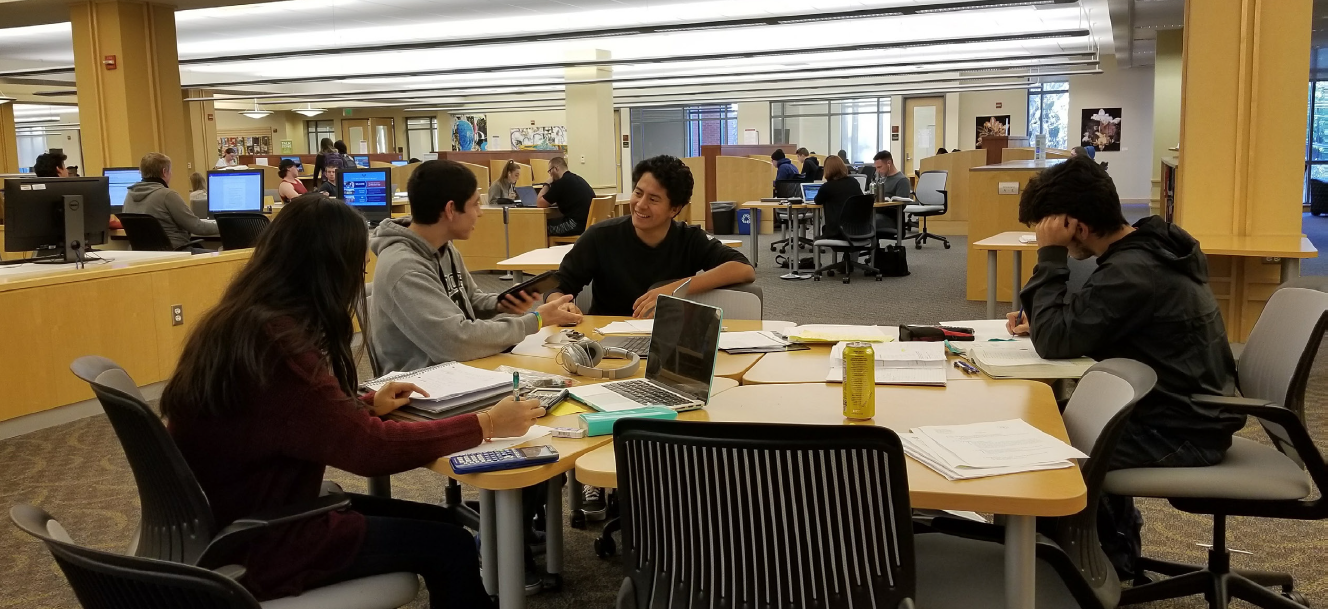
\includegraphics[width = 1.0\textwidth]{images/SRJC Tutorial Center.PNG}
	\end{center}
\end{frame}
		
\subsection{Empire College \& The Wine Industry}
	\begin{frame}
	\frametitle{Empire College and the Hotels/Hospitality Industry}
	\begin{itemize}
		\item After backpacking around Europe for 4 months I decided to work in the Hotels and Hospitality Industry.
\item I attended Empire College's Hospitality, Travel, Hotels and Wine Industry program
\item This was during the Great Recession, when everyone was firing not hiring, and I was not able to get hired by any hotels.
\end{itemize}
\begin{center}
	
\includegraphics[width = 1.0\textwidth]{images/Empire College.png}
\end{center}
\end{frame}

\begin{frame}
	\frametitle{The Wine Industry and Hospitality}
	\begin{itemize}
	\item I was able to get hired by the Wine Industry!
	\item Poured wine for Rosenbloom, J, and Murphy-Goode Wineries.
	\item Harvest Cellar Worker for Martinelli Winery.
\end{itemize}
\begin{center}
	\includegraphics[width = 1.0\textwidth]{images/wine science.png}
\end{center}
\end{frame}

		\subsection{Humboldt State University \& Academic Research}
		\begin{frame}
		\frametitle{Humboldt State University}
	\begin{itemize}
		\item I returned to the SRJC to study Chemistry and Oenology (The Scientific Study of Wine Making).
\item Yet I preferred studying math, and wanted to do research.
\item Transferred to Humboldt State University
\item Major:   Psychology
\item Minors:  Applied Statistics, and Applied Mathematics
\end{itemize}
\begin{center}
	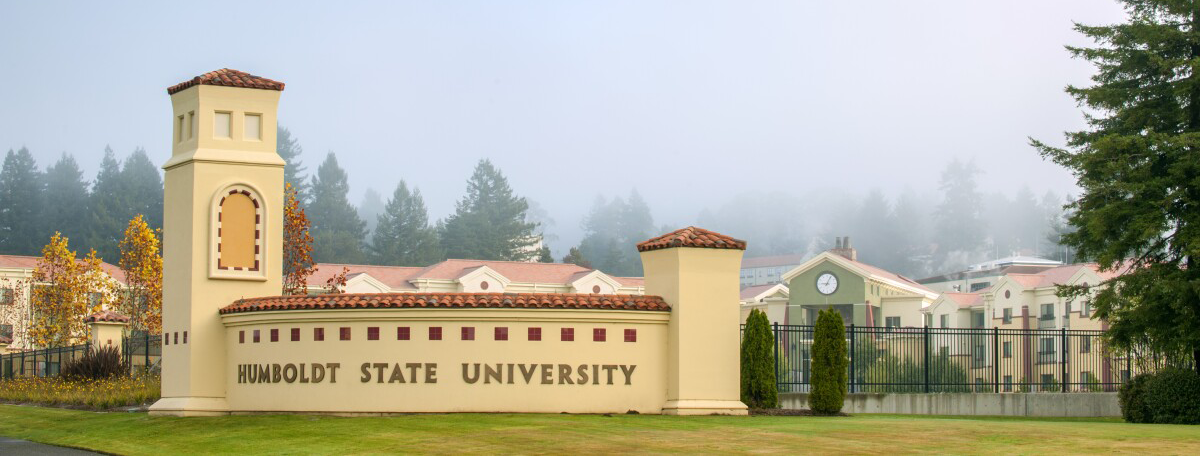
\includegraphics[width = 1.0\textwidth]{images/HSU.PNG}
\end{center}
\end{frame}

		\begin{frame}
	\frametitle{Academic Research}
	\begin{itemize}
		\item Completed 2 pieces of undergraduate research as the only author:  
		\item Reliability and Validity of the Health Efficacy Scale for College Students
		\item An Examination of Perfectionism and Body Esteem on the Eating Patterns of Male and Female College Students
		\item Found that I preferred to do the statistics and data analysis, and not the actual research.  
	\end{itemize}
	\begin{center}
		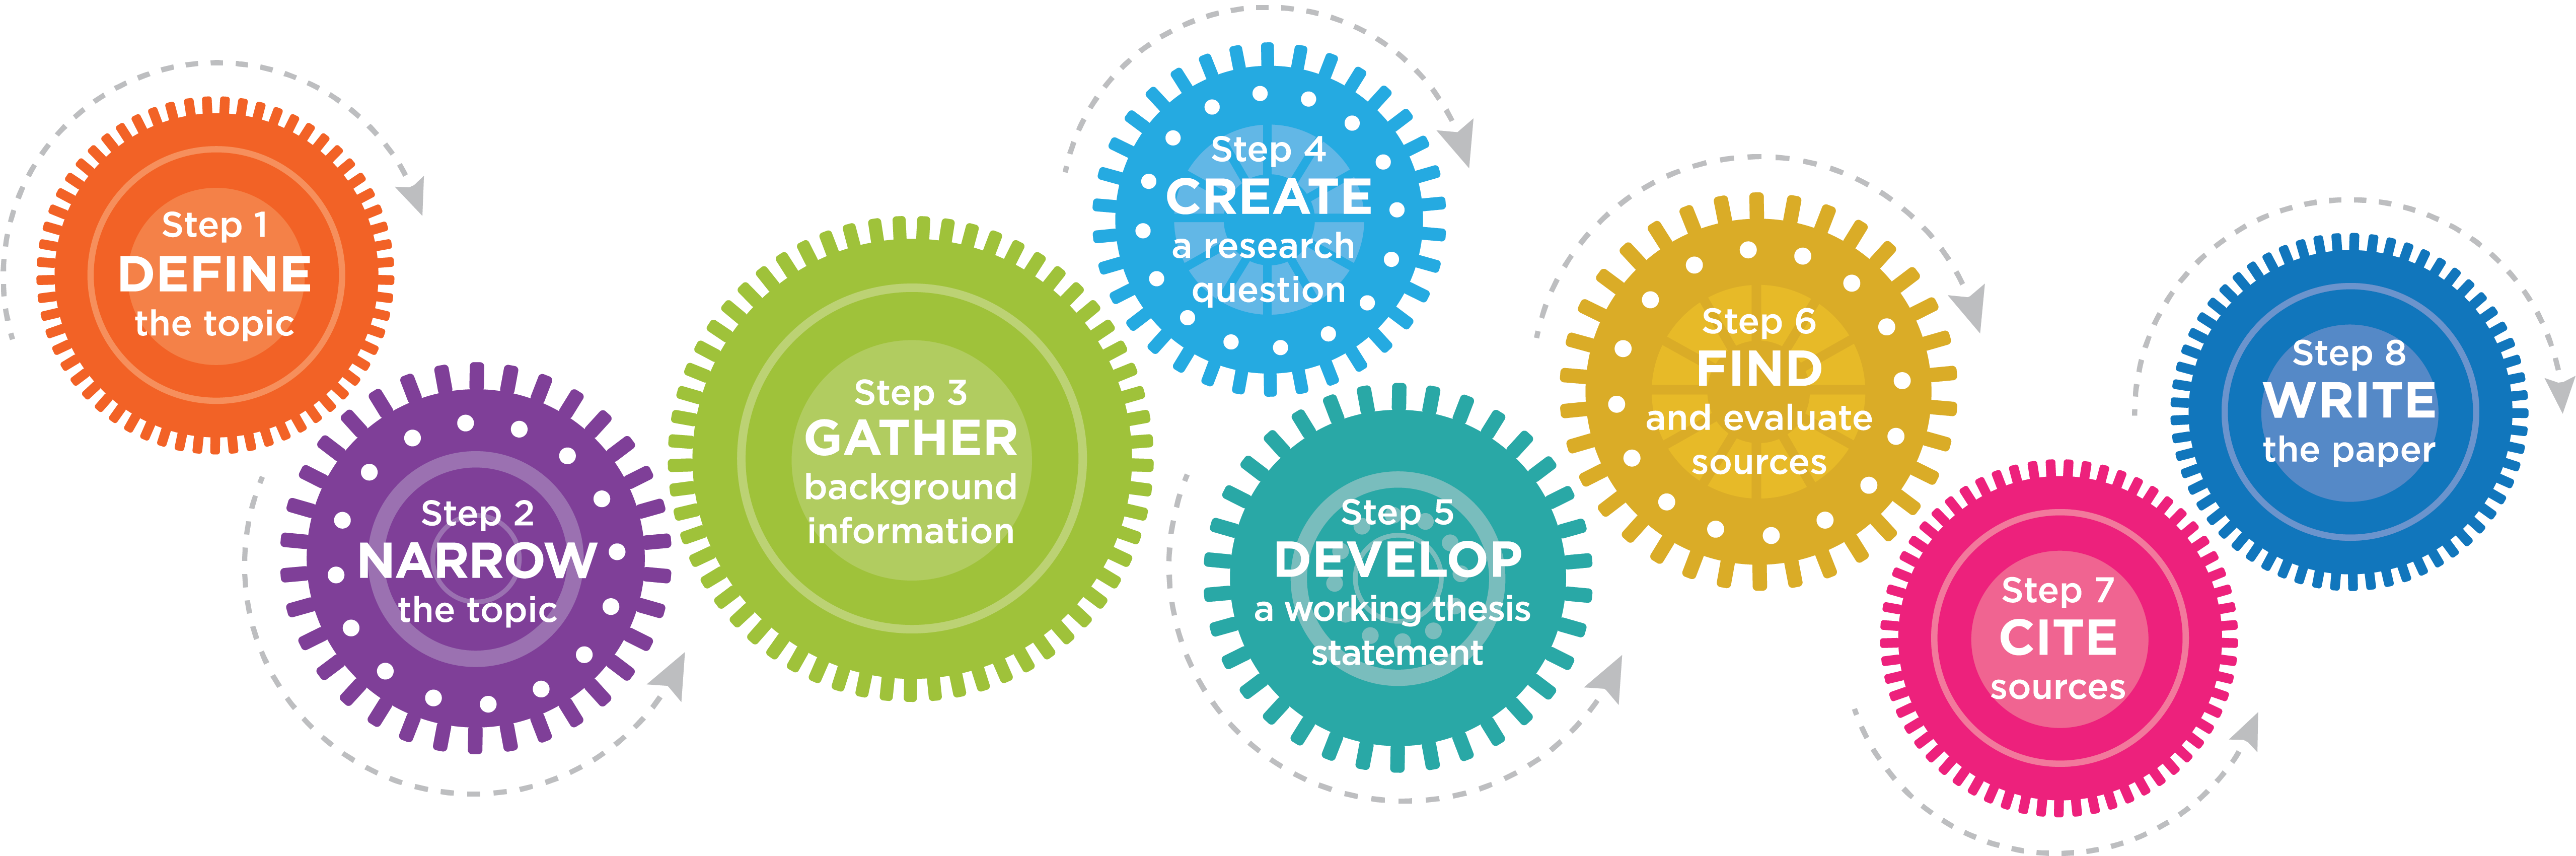
\includegraphics[width = 1.0\textwidth]{images/Research-process.png}
	\end{center}
\end{frame}

		\subsection{Santa Rosa Junior College \& Web Development}
				\begin{frame}
			\frametitle{Santa Rosa Junior College, Cancer, and Japan}
	\begin{itemize}
		\item My fiancee (now wife) was in Japan. 
		\item Father was slowly passing away from cancer in Santa Rosa.
\item So I returned to the SRJC to study Computer Science and Web Development.
\item I would spend one semester in Santa Rosa, and the other in Nagoya studying online.
\item Additional subjects included:  Interactive Multimedia, Mathematics, Adobe PhotoShop, Project Management, Microsoft Excel, Business Management, Game Programming.
\end{itemize}
\begin{center}
	
\includegraphics[width = 1.0\textwidth]{images/web dev.png}
\end{center}
\end{frame}

		\subsection{Johns Hopkins University \& Teaching}
\begin{frame}
	\frametitle{Johns Hopkins University and Data Science}
				\begin{itemize}
		\item My wife and I were planning to move out to Texas, and for me to start a new career in Data Analysis, or Web Development.
\item But this was in the Spring of 2020... 
\item So we moved to Fort Bragg and I applied to a Graduate School.
\item I was accepted into Johns Hopkins Universities Whiting School of Engineering's Masters of Science program in Data Science.
\end{itemize}
\begin{center}
	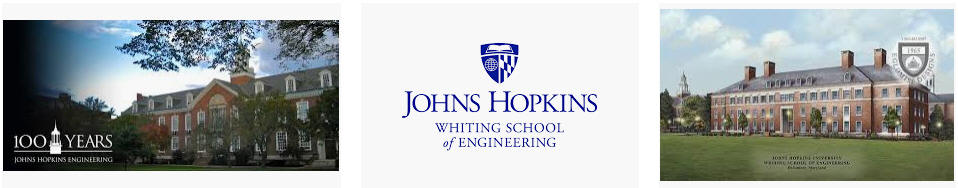
\includegraphics[width = 1.0\textwidth]{images/Johns_83.jpg}
\end{center}
\end{frame}

\begin{frame}
	\frametitle{Tutoring and Teaching at Mendocino College}
	\begin{itemize}
		\item My wife started taking Art Classes at Mendocino College in the Fall of 2021.  
		\item So one time I submitted a general application, and was eventually hired to be an embedded tutor for Applied Mathematics and Statistics, for Spring 2022.
		\item During the Summer I was hired to be an instructor in computer science, \& then in digital arts and media.
		\item Making Fall 2022 my first semester as a college instructor.  
	\end{itemize}
	\begin{center}
		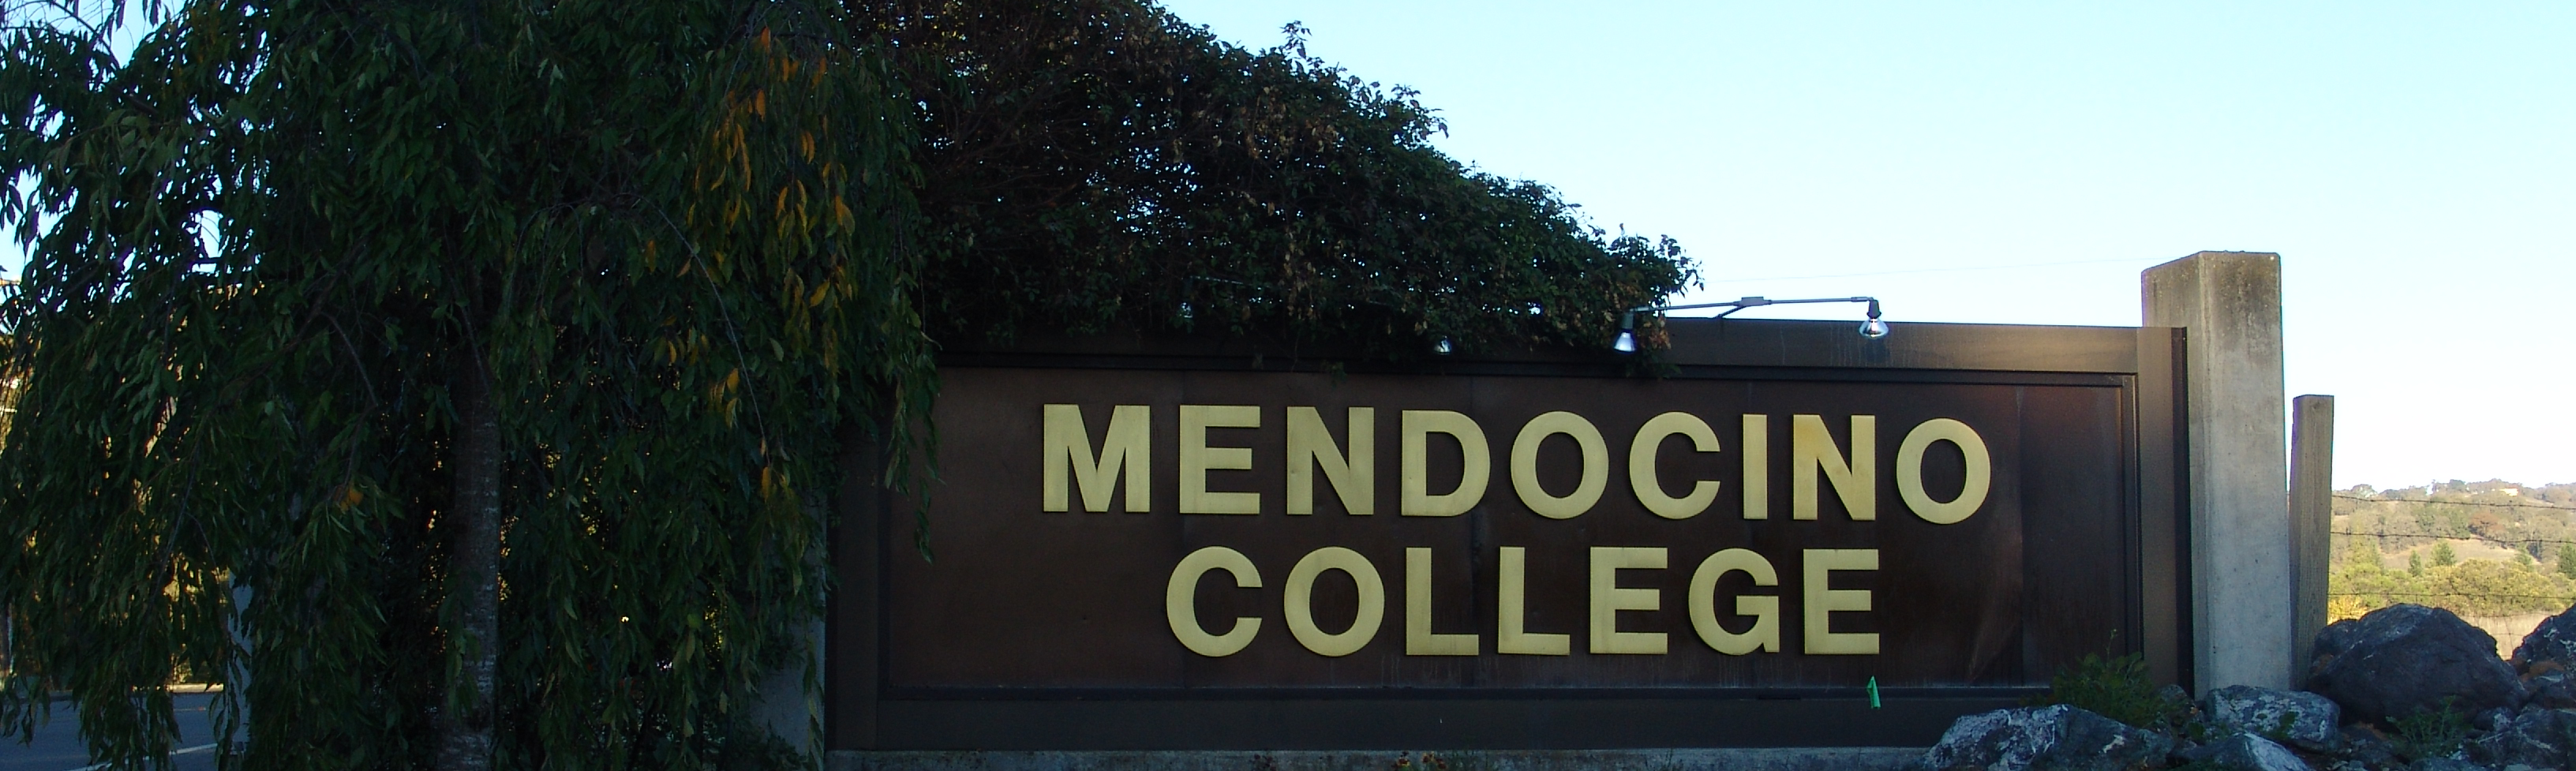
\includegraphics[width = 1.0\textwidth]{images/MENDOCINO_COLLEGE.png}
	\end{center}
\end{frame}


	\section{Hobbies \& Interests}
		\subsection{Computers, Programming \& Gaming}
			\begin{frame}
	\frametitle{Computers}
\begin{itemize}
	\item My first computer was given to me by my Father, it was an old Amiga system.
	\item My family as online with dial-up in 1995, less than a year after the first website was ever launched.  
	\item I have always been fascinated by computers and the internet.
	\item Started repairing computers as a side job as early as 15.   
\end{itemize}
\begin{center}
	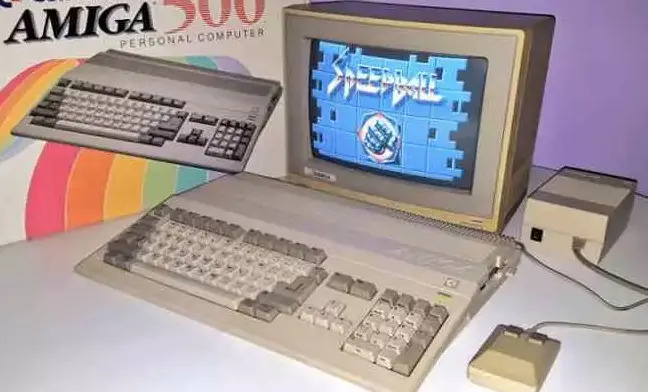
\includegraphics[width = 1.0\textwidth]{images/Amiga-Computer.jpg}
\end{center}
			\end{frame}
		
\begin{frame}
	\frametitle{Programming}
	\begin{itemize}
		\item Started programming casually, not even realizing I was actually programming.  
		\item EasyUO was my first programming experience, making scripts for an MMO game I played.  
		\item After that I learned HTML and how to write nested-IF functions in Excel.
		\item Now I have experience programming in:  R, Python, Java, SQL, HTML5, CSS3, JavaScript, C++
	\end{itemize}
	\begin{center}
		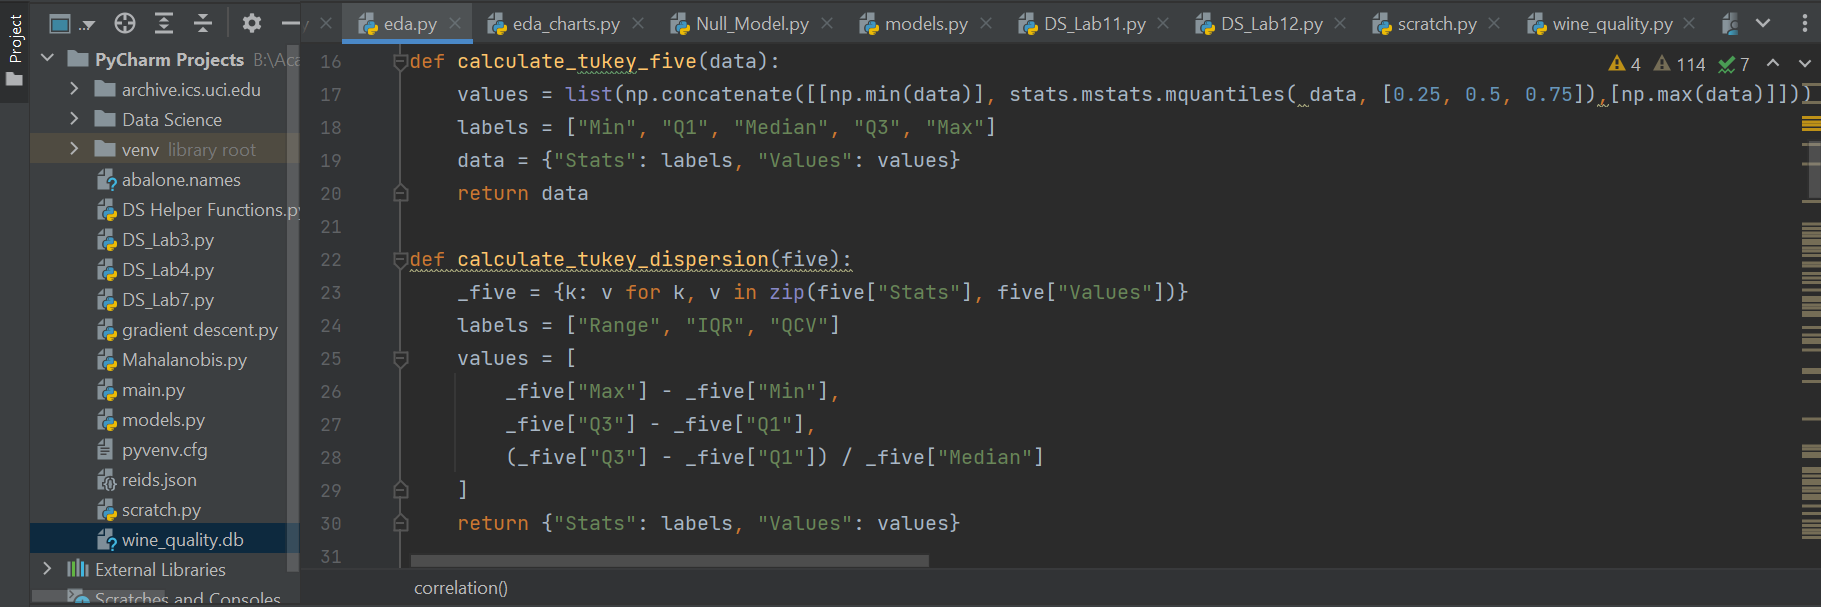
\includegraphics[width = 1.0\textwidth]{images/programming.png}
	\end{center}
\end{frame}
		
\begin{frame}
	\frametitle{Board Games}
	\begin{itemize}
		\item I've always loved board games, from as early as I can remember. 
		\item My favourite board games include:
		\item Risk
		\item Monopoly
		\item Settlers of Catan
	\end{itemize}
	\begin{center}
		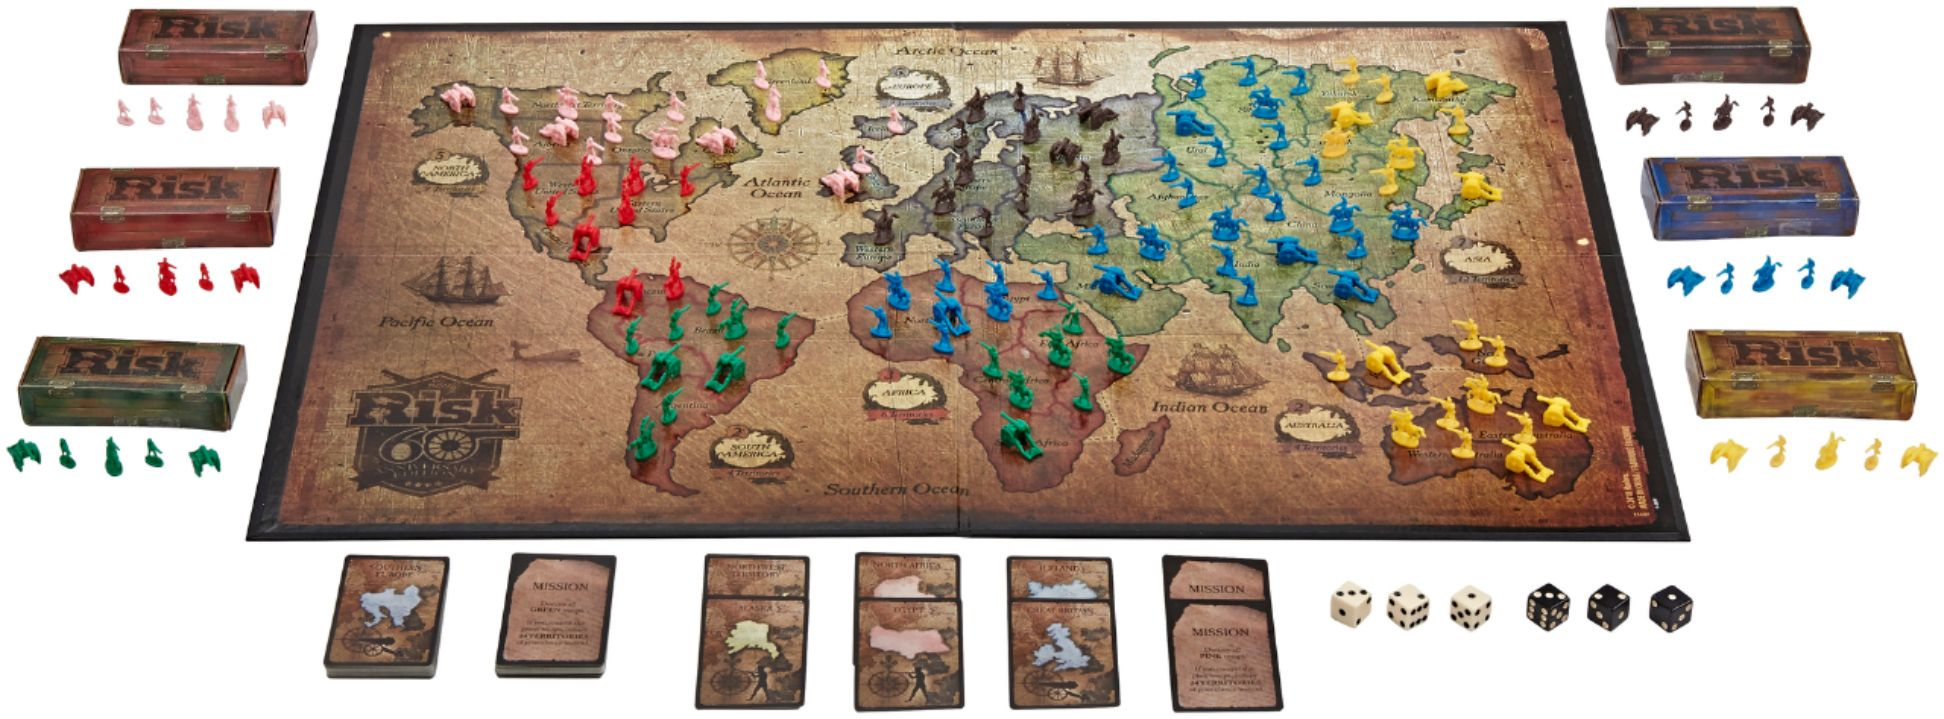
\includegraphics[width = 1.0\textwidth]{images/risk.jpg}
	\end{center}
\end{frame}

\begin{frame}
	\frametitle{Card Games}
	\begin{itemize}
		\item Magic: The Gathering
		\item Poker: Texas Hold'em
	\end{itemize}
	\begin{center}
		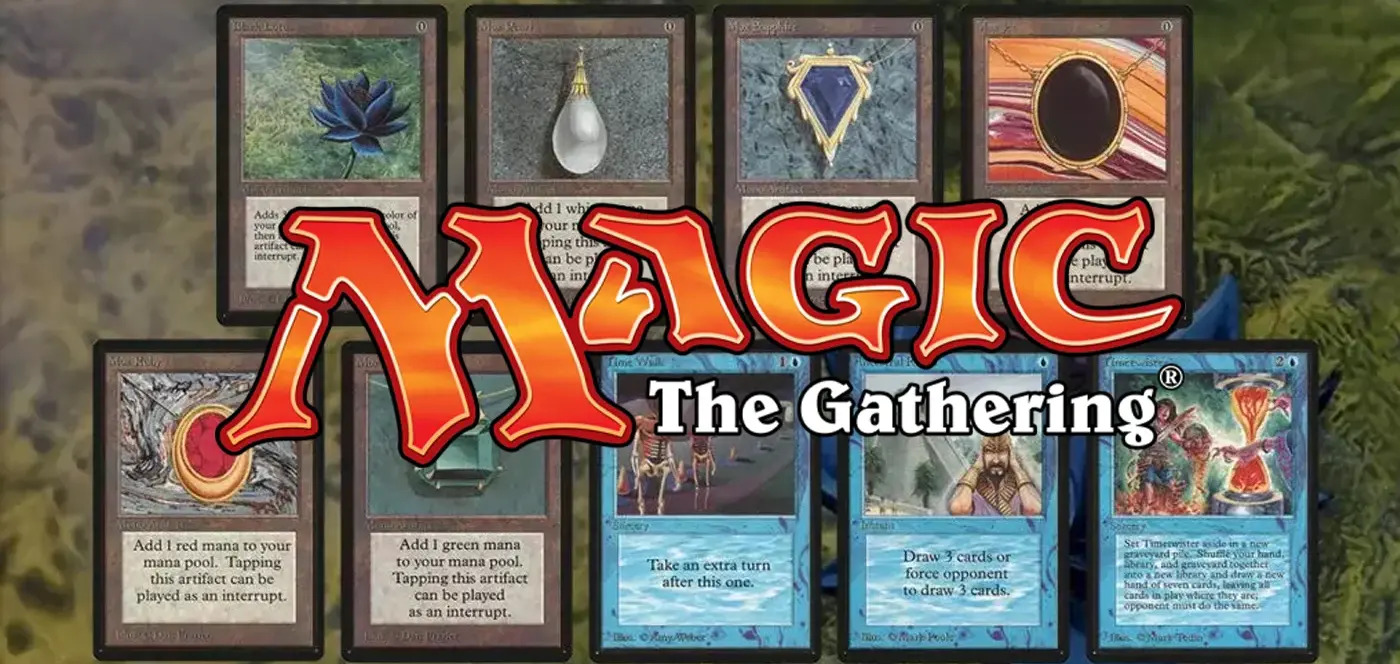
\includegraphics[width = 1.0\textwidth]{images/mtg.jpg}
	\end{center}
\end{frame}

\begin{frame}
	\frametitle{Video Games}
	\begin{itemize}
		\item SNES:  EarthBound \& Chrono Trigger
		\item PC:    Ultima Online, Baldur's Gate
	\end{itemize}
	\begin{center}
		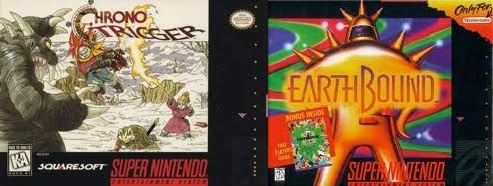
\includegraphics[width = 1.0\textwidth]{images/snes.jpg}
	\end{center}
\end{frame}
		
				\subsection{Generative Artwork \& NFTs}
\begin{frame}
	\frametitle{Cryptocurrency, Generative Artwork \& NFTs}
	\begin{itemize}
		\item I knew of bitcoin, litecoin, ripple and dogecoin when they were first made, but I didn't get into crypto until 2017.
		\item In 2021 I became interested in NFTs, as a way to publish artwork individually without agents or dealers.
		\item This is when I first started to create generative artwork, by making algorithms in R \& Python.
		\item Biggest sale has been an NFT on OpenSea.io for over \$700.  
	\end{itemize}
	\begin{center}
		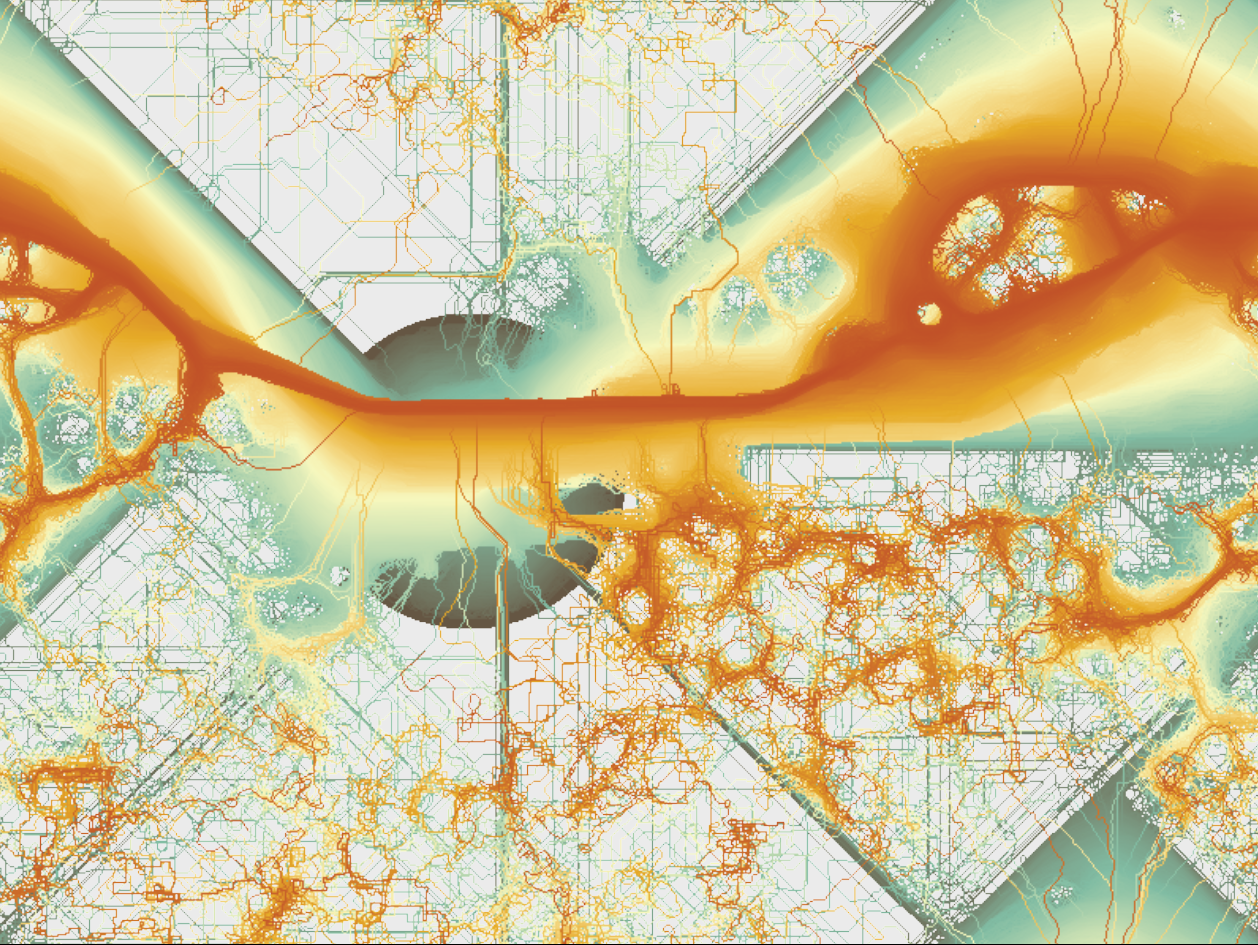
\includegraphics[width = 0.5\textwidth]{images/first cover.png}
	\end{center}
\end{frame}

\subsection{Fencing \& Circus}
\begin{frame}
	\frametitle{North Bay Fencing Academy}
	\begin{itemize}
		\item Started fencing at the Santa Rosa Junior College when I was 15 years old.
		\item Competed in a few UC fencing tournaments.
		\item Continued fencing at the North Bay Fencing Academy.
		\item Fenced occasionally in Humboldt at various locations.
	\end{itemize}
	\begin{center}
		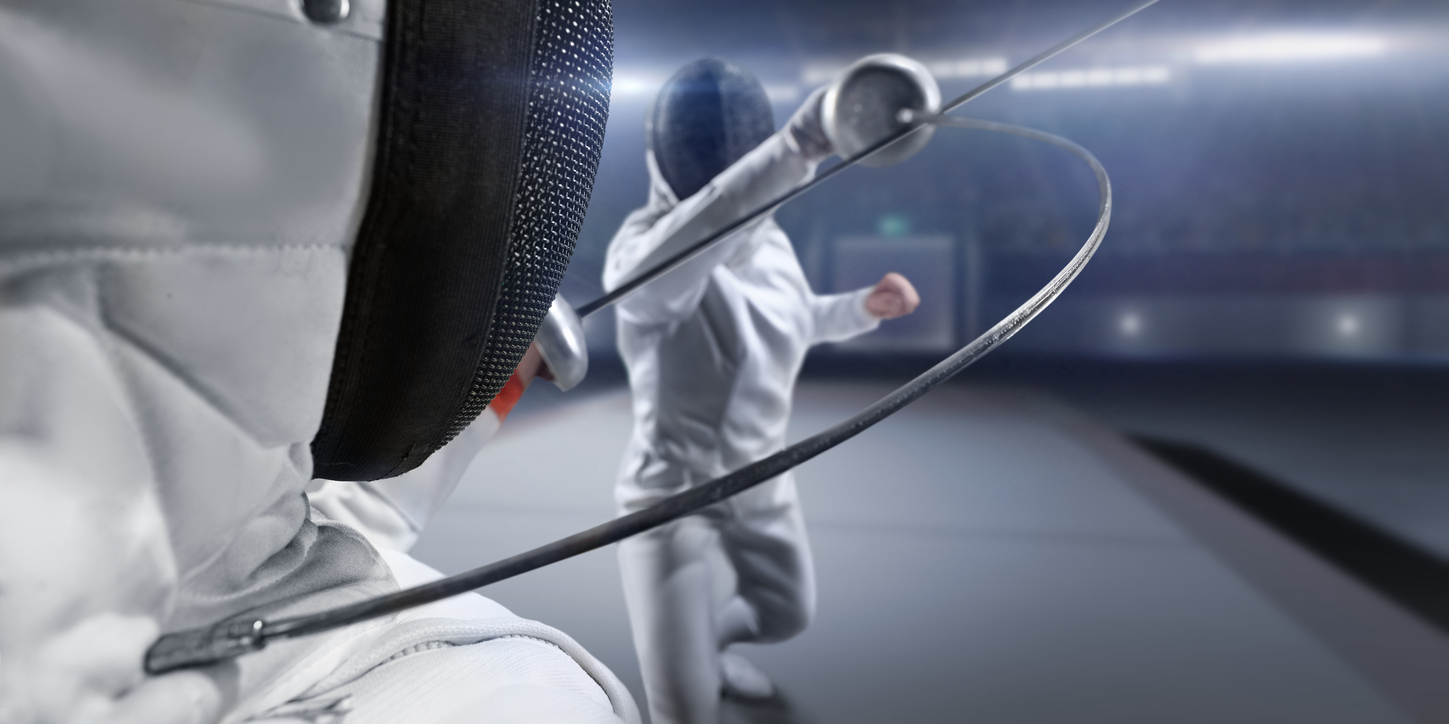
\includegraphics[width = 1.0\textwidth]{images/fencing.jpg}
	\end{center}
\end{frame}

\begin{frame}
	\frametitle{Humboldt Circus}
	\begin{columns}
		\column{.6\textwidth}
	\begin{itemize}
		\item A friend from home transferred to HSU before me, and he got me into the Humboldt Circus.
		\item I had never been on stage before this.
		\item My Toys:  Yo-Yo, Diabolo, Spinning Tops, Juggling
	\end{itemize}
		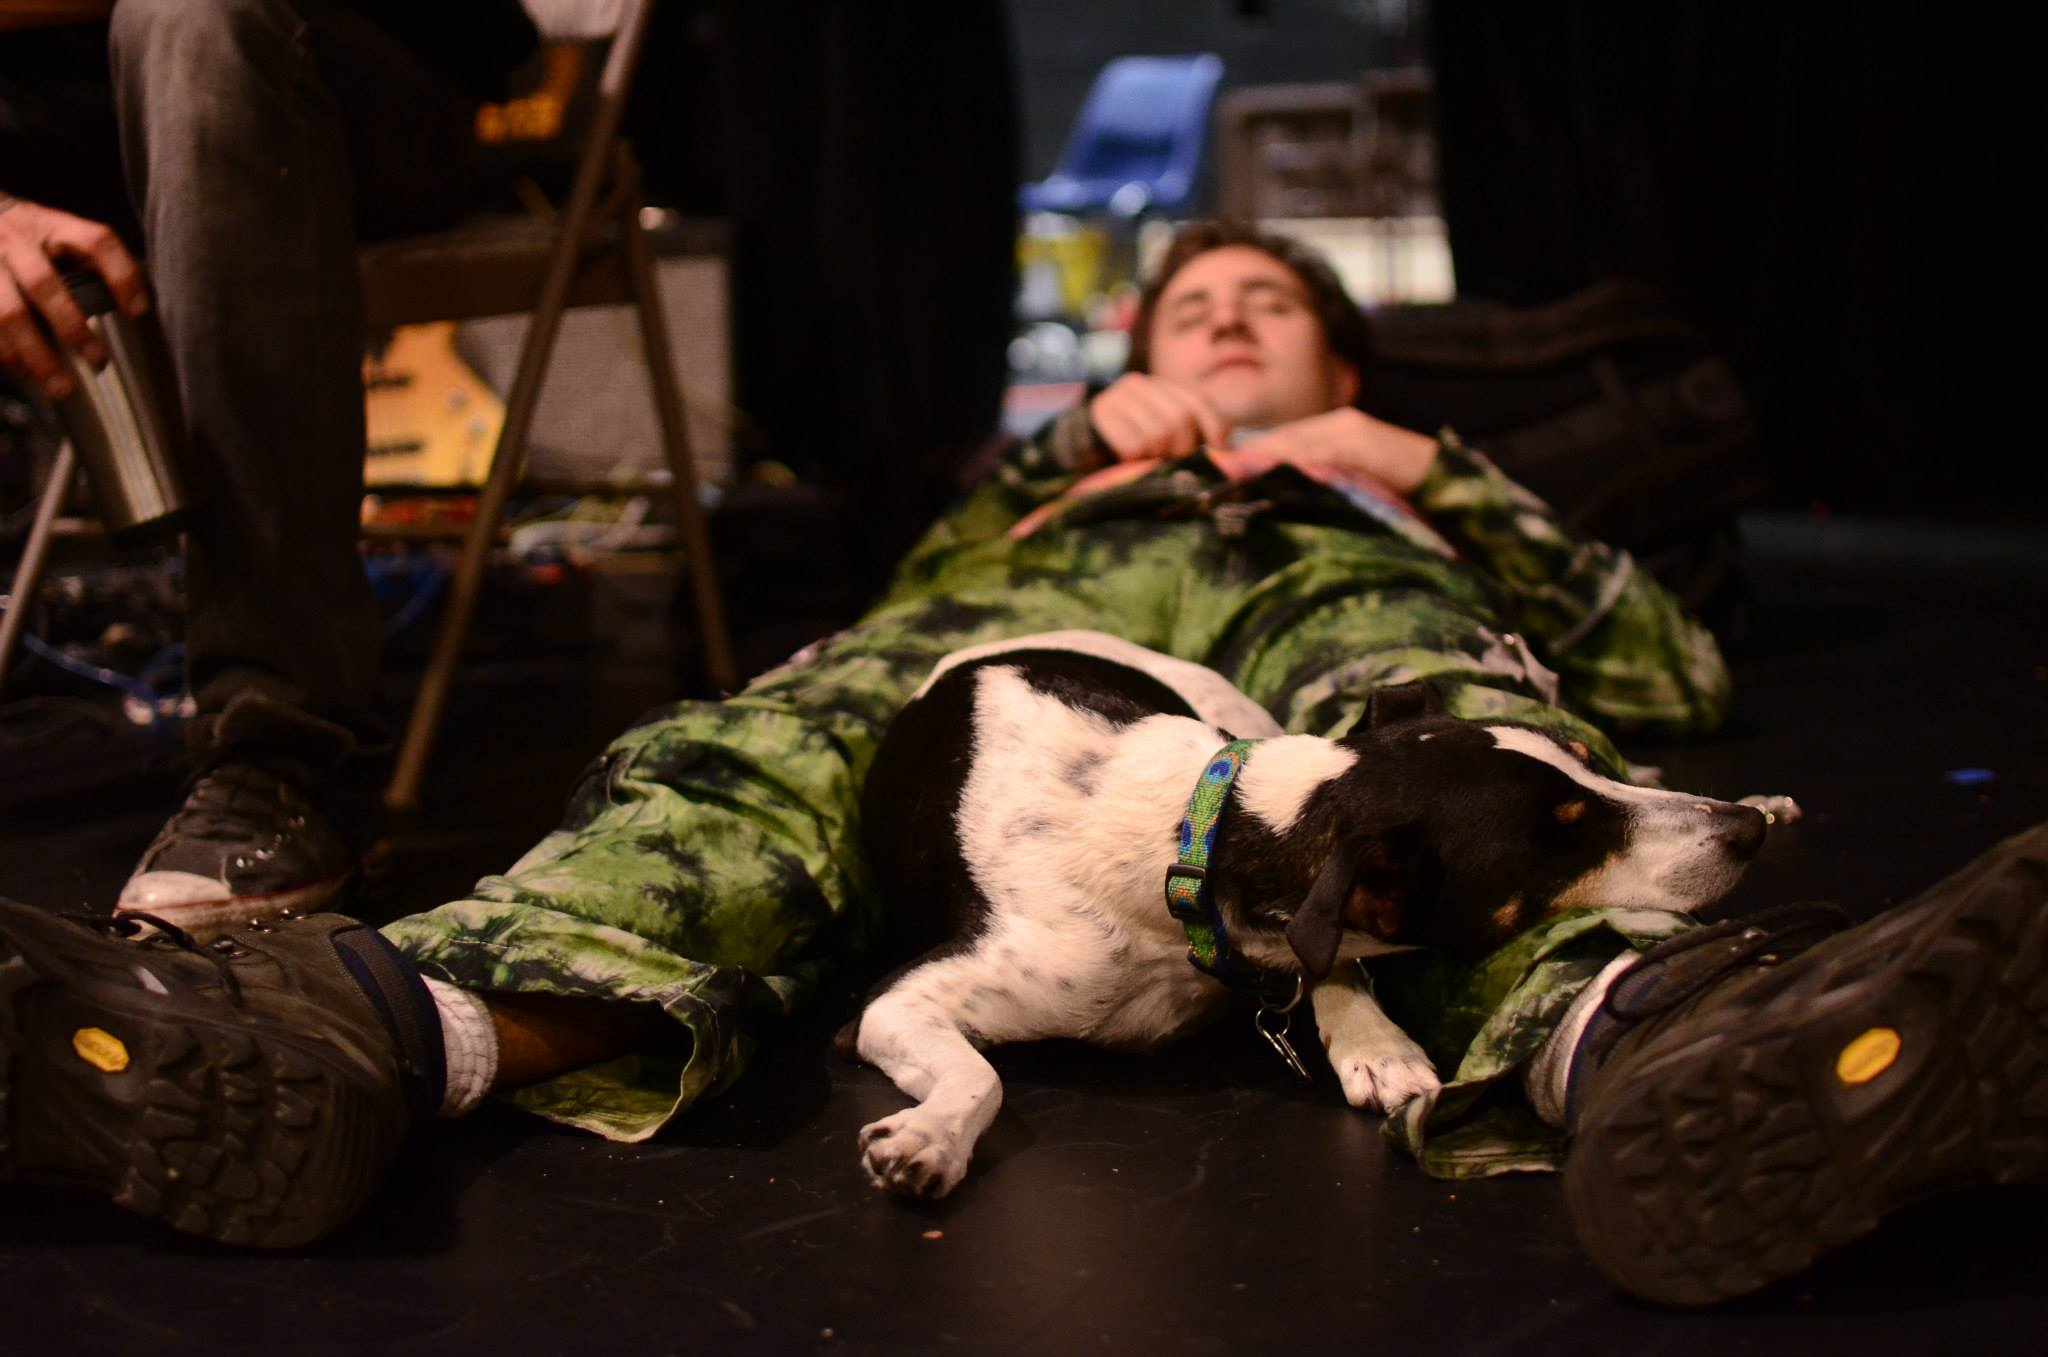
\includegraphics[width = 1.0\textwidth]{images/1410944_10100133942385529_1241810700_o.jpg}
\column{.5\textwidth}
\begin{center}
		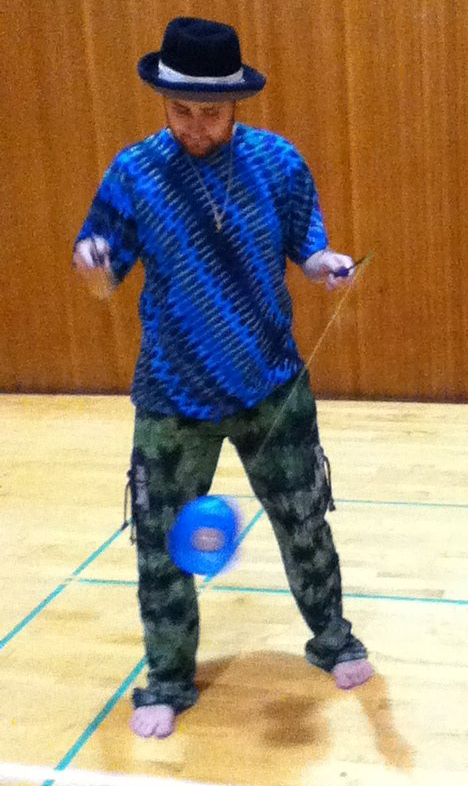
\includegraphics[width = 0.9\textwidth]{images/circus diabolo.png}
		\end{center}
	\end{columns}
\end{frame}
		
		\subsection{Hiking, Camping, \& Nature}
\begin{frame}
	\frametitle{Hiking, Camping, Nature \& Scouts}
	\begin{itemize}
		\item I'm an Eagle Scout.  
		\item Traveled around parts of the USA, Europe and Asia with various Scout Troops, as a scout and assistant scoutmaster.
		\item I love hiking, swimmable rivers and disperse camping.
	\end{itemize}
	\begin{center}
		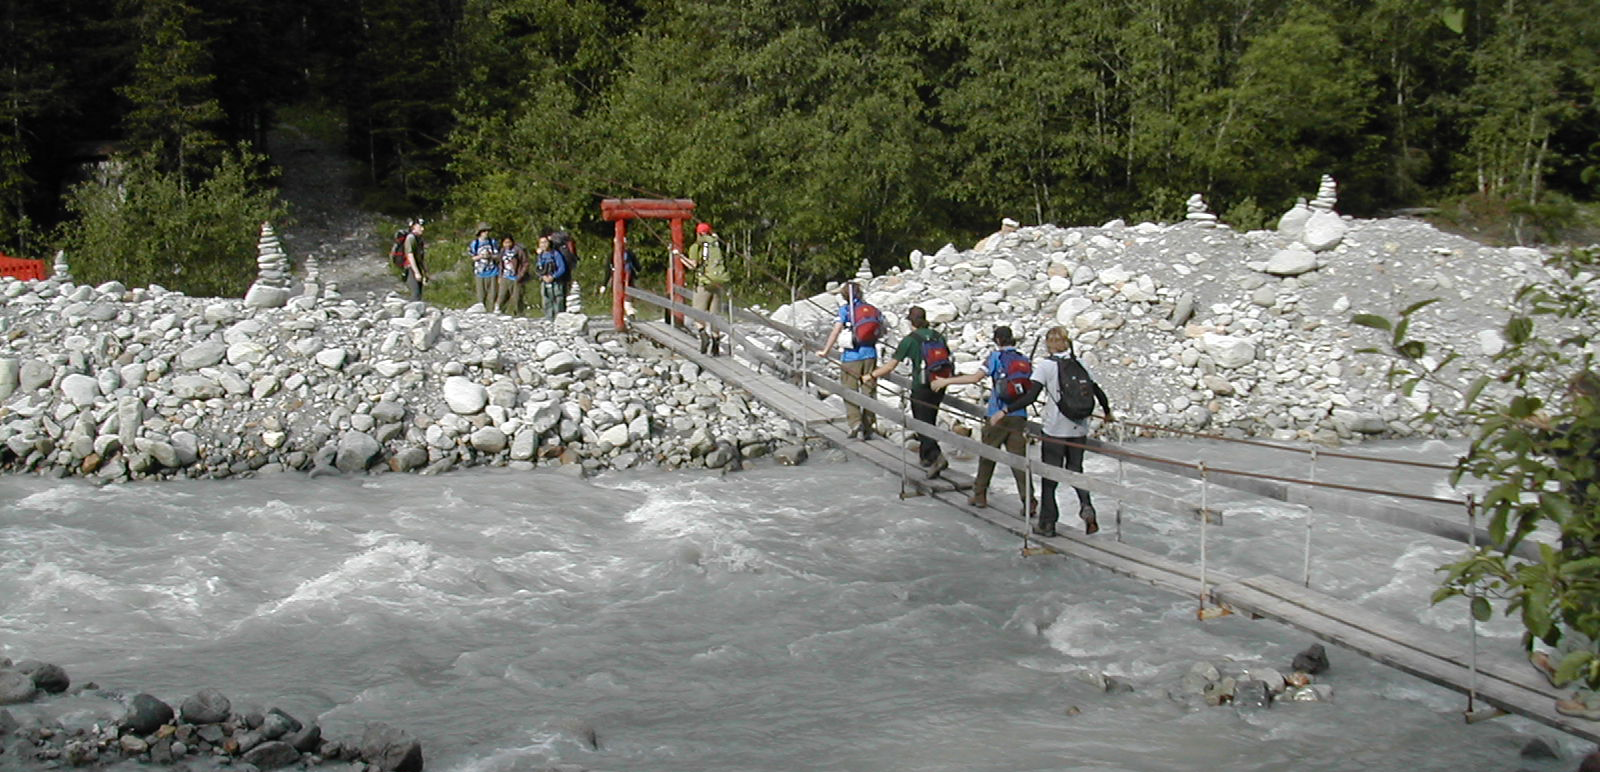
\includegraphics[width = 1.0\textwidth]{images/scouts.png}
	\end{center}
\end{frame}
	
		\subsection{Traveling \& Backpacking}
\begin{frame}
	\frametitle{Travel Experiences}
	\begin{itemize}
		\item I've been to over 30 individual countries.
		\item Countries I've visisted twice:  Denmark, Finland, Ireland, Thailand
		\item Countries I've visited 3 or more times:  Japan, China.
	\end{itemize}
	\begin{center}
		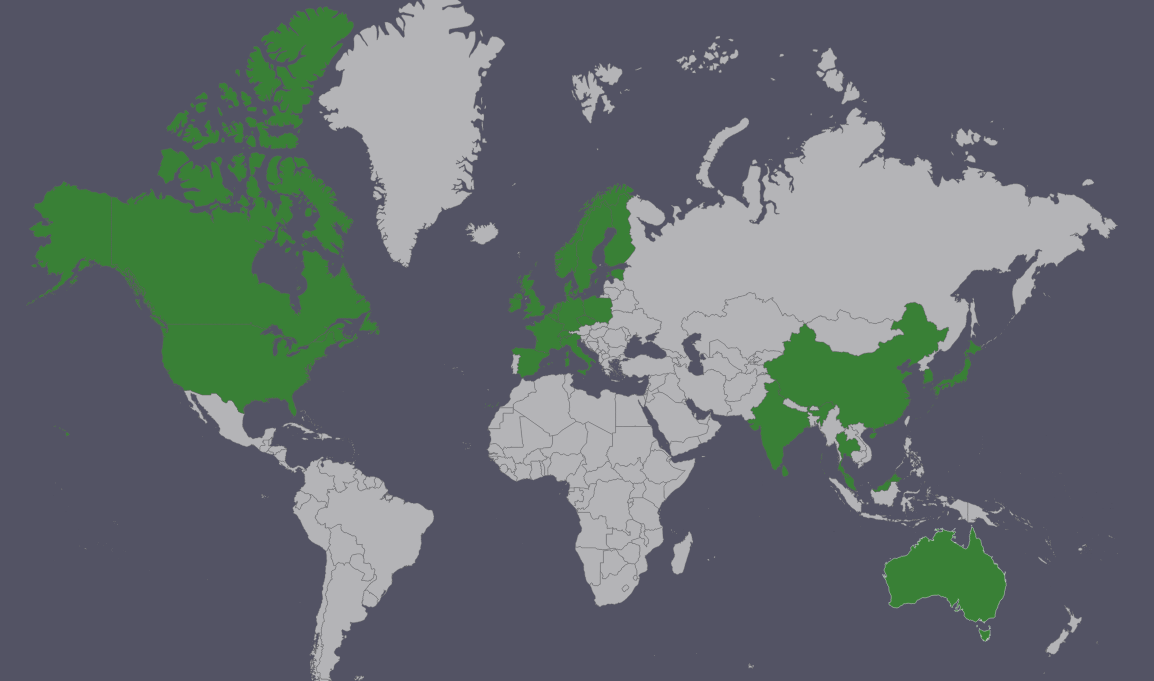
\includegraphics[width = 0.9\textwidth]{images/countries visited.png}
	\end{center}
\end{frame}


	\section{Future Plans}
	
\subsection{Children \& Family}
\begin{frame}
	\frametitle{Children \& Family}
	\begin{itemize}
		\item My wife and I hope to have our first child next year.
		\item We hope for a family with 3 children.  
		\item Eventually we want to add some cats and ducks to our family.  
	\end{itemize}
	\begin{center}
		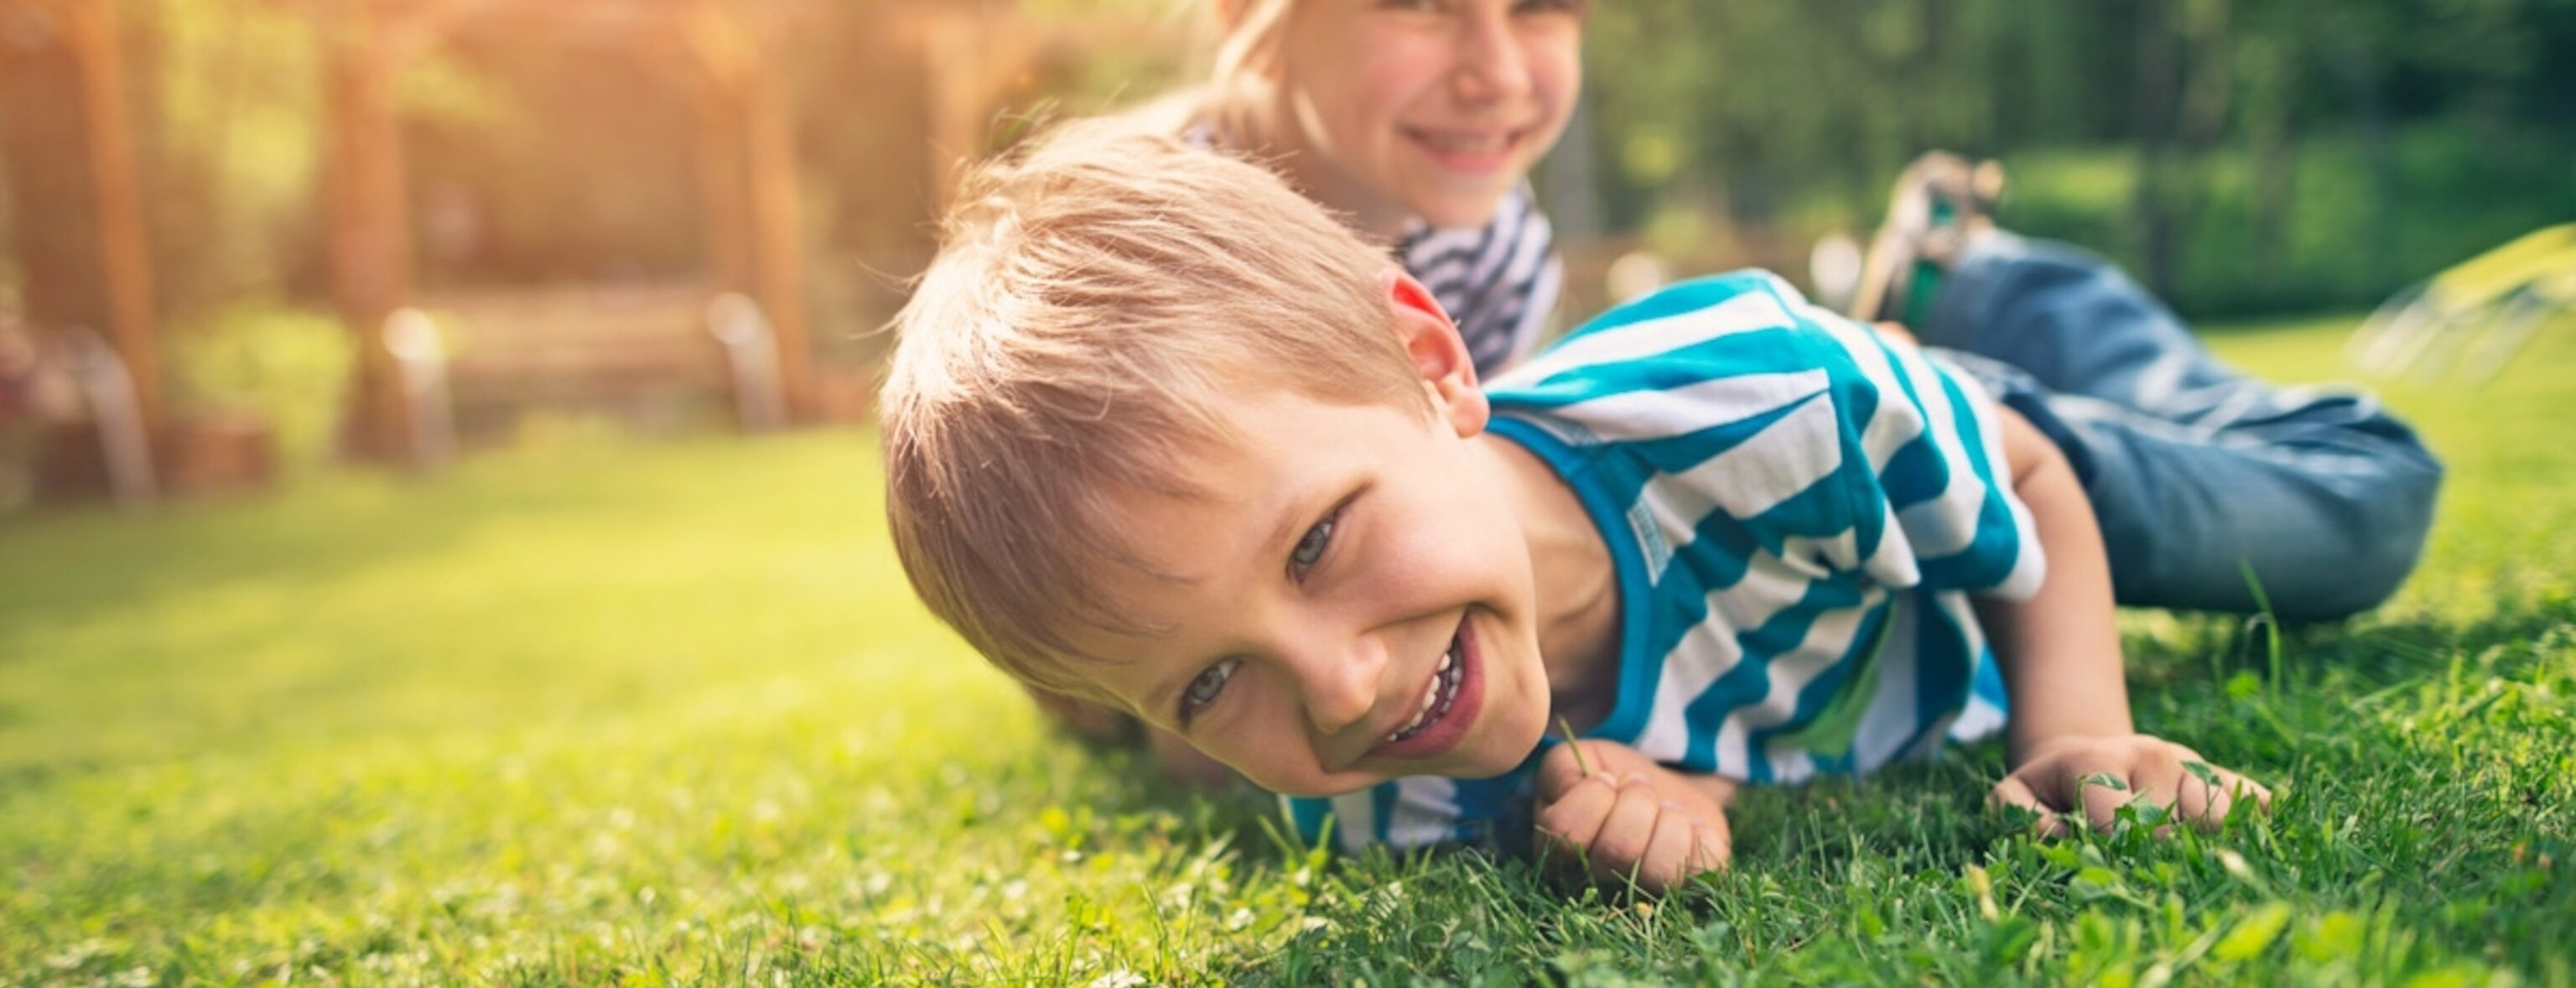
\includegraphics[width = 1.0\textwidth]{images/kids.jpg}
	\end{center}
\end{frame}

\subsection{Campground \& Business}
\begin{frame}
	\frametitle{Campground \& Business}
	\begin{itemize}
		\item We have a special variety of raspberry which is white, delicious, and grows wonderfully on our property.
		\item So we are creating our own company:  White Berry Farm
		\item We will provide camping through AirBnB and HipCamp
		\item Along with selling fruits and plants from our orchard.
	\end{itemize}
	\begin{center}
		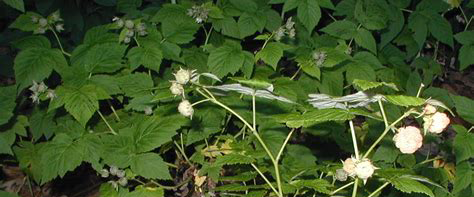
\includegraphics[width = 1.0\textwidth]{images/white raspberry.png}
	\end{center}
\end{frame}

\subsection{Gaming Industry \& High-Tech}
\begin{frame}
	\frametitle{Gaming Industry \& High-Tech}
	\begin{itemize}
		\item The "silicon valley of gaming" is in Marin County.
		\item Cryptocurrency and NFTs are the future of online gaming.
		\item The gaming industry incorporates many of the skills which I have, such as: Programming, Graphic Arts, Web Development, Data Science, Artificial Intelligence.  
	\end{itemize}
	\begin{center}
		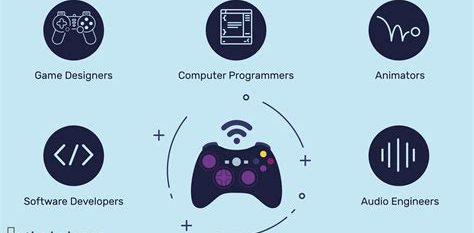
\includegraphics[width = 0.95\textwidth]{images/game industry.png}
	\end{center}
\end{frame}

\subsection{Graduation \& PhD}
	\begin{frame}
		\frametitle{Graduate School \& PhD}
		\begin{itemize}
			\item Finish my Masters Degree in Data Science.  
			\item Slowly study for a PhD in Artificial Intelligence from Johns Hopkins University.  
		\end{itemize}
					\begin{center}
		
\includegraphics[width = 1\textwidth]{images/ai banner.jpg}
	\end{center}
	
	\end{frame}


	\section{}	
		\subsection{End Card}
	\begin{frame}
		\frametitle{End Card}	
		\begin{columns}
			\column{.6\textwidth}
			\vspace{-25pt}
			\begin{itemize}
				\item Joshua Paul Barnard
				\item Computer Science Instructor
				\item Mendocino College
			\end{itemize}
			\begin{itemize}
				\item This Presentation was made in \LaTeX
				\item For the Fall 2022 semester.  
			\end{itemize}
			\begin{itemize}
				\item jbarnard@mendocino.edu
				\item github.com/JoshuaPaulBarnard
			\end{itemize}
			\column{.45\textwidth}
			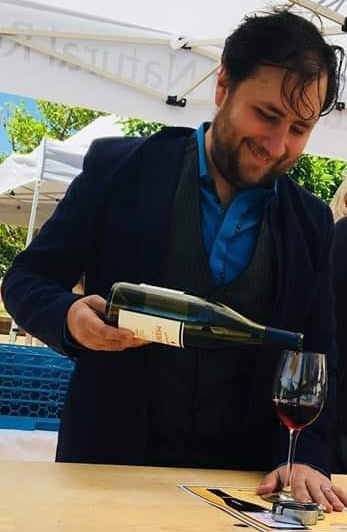
\includegraphics[width=.85\textwidth]{images/shone farm wine pouring - vert.png}
		\end{columns}
	\end{frame}
	
\end{document}